% allocate 9 pages
\chapter{Evaluation}
Compare the compute requirements? (Auto prompting is computationally expensive)

Compare the scalability with an increase in class numbers? (Auto promptig not scalable)
\section{Success Criteria}
\subsection{Core Project}
The project will be considered a success if it achieves the following:
\begin{itemize}
    \item Preprocess datasets MNLI and QNLI so that they are suitable for the downstream task textual-entailment-based question answering.
    \item Reimplement a \textbf{manual discrete prompt-based} model, which involves carefully designing several appropriate prompts manually, and then quantitatively comparing the performance of using different prompts.
    \item Reimplement an \textbf{automated discrete prompt-based} model, which involves applying a published automated template generation method, then evaluate and compare its performance against the manual discrete prompt-based model.
    \item Reimplement a \textbf{differential prompt-based} model and analyse its performance by comparing it with both automated and manual discrete prompt-based models.
    \item Launch backdoor attacks onto the PLM of the three prompt-based models and evaluate the performance of each attack. Various backdoor triggers would be designed, and the effectiveness of each would be analysed. These design choices include the word choice, the length of the word, the insertion position of the triggers and the poison ratio of the dataset.
\end{itemize}

\subsection{Extensions}
In the context of classification downstream tasks, precision-at-n could be suited to measure the performance of the prompt-based models. When a prompt-based model fills the mask token with a word, it would first rank the possible words by their probabilities, and precision-at-n is defined as the percentage of the top-n words that leads to correct classification. In this project, we will use precision-at-1 (P@1) and precision-at-10 (P@10) as metrics.

For analysing the performance of the backdoor attack on each prompt-based model, the two primary metrics are:
\begin{itemize}
    \item Attack success rate (ASR): the percentage of the poisoned samples that the model misclassified due to the backdoor attack.
    \item Accuracy: the proportion of samples the model can still classify correctly, which ensures that the model performs normally under scenarios where the triggers are not present.
\end{itemize}
\paragraph{An additional downstream task}
 For this downstream task, a manual discrete, automated discrete and differential prompt-based model can be constructed. After launching backdoor attacks onto those prompt-based models, a case study can be carried out to compare and analyse the impacts of backdoor attacks on different downstream tasks (e.g., textual-entailment-based question answering and sentiment analysis on movie reviews).

 \paragraph{Invisible backdoors using Unicode characters}
 The backdoor attacks using nonsense words cannot preserve the semantic meaning of the sentences and are distinguishable under careful inspection. Unicode-encoded characters that are imperceptible to the human eye can be designed \cite{Boucher21}. Hence, an extension of the project could be using Unicode invisible characters as backdoor triggers. 

 \paragraph{Backdooring onto the trainable prompts}
 The published backdoor attacks inject poisoned prompts when training the PLM. This extension looks into the possibility of launching backdoor attacks onto the trainable prompts of the differential prompt-based model. 

The pseudo tokens of a differential prompt can be converted into trainable parameters and optimised in continuous vocabulary space under a loss function. Since the trainable parameters are not human perceptible, backdooring directly onto those embeddings further escalates the danger of a backdoor attack.


% \begin{table*}[!ht]
\centering
\adjustbox{max width=\hsize}{
	\begin{tabular}{c | llll | llll }
	\toprule
	\multicolumn{1}{c}{ }                      
	& \multicolumn{4}{c}{SST2}                      
	& \multicolumn{4}{c}{QNLI} \\
	$K$ 
        & Baseline & Auto	& Diff	& Manual 
	& Baseline & Auto	& Diff	& Manual \\
	\midrule
	$16$   
	% SST2
	& $72.1 \pm 15.0$        
	& $70.1 \pm 3.9$           
	& $\boldsymbol{87.8 \pm 0.7}$
	& $\underline{86.9 \pm 1.6}$           

	% QNLI 
	& $49.9 \pm 0.2$        
	& $53.4 \pm 1.3$           
	& $\underline{59.5 \pm 3.6}$             
	& $\boldsymbol{74.1 \pm 1.2}$           

	\\
	$100$  
 	% SST2
	& $\boldsymbol{89.6 \pm 0.5}$             
	& $83.5 \pm 4.3$              
	& $88.6 \pm 0.7$            
	& $\underline{89.4 \pm 1.0}$       
        % QNLI
        & $78.9 \pm 2.3$
        & $74.0 \pm 4.3$
        & $\underline{80.2 \pm 2.1}$
        & $\boldsymbol{82.7 \pm 0.7}$
        \\
	$1000$
        % SST2
	& $\boldsymbol{92.7 \pm 0.2}$           
	& $\underline{92.5 \pm 0.2}$
        & $90.1 \pm 0.7$
        & $92.3 \pm 0.2$
        % QNLI
        & $\underline{87.2 \pm 1.0}$
        & $83.2 \pm 3.8$
        & $85.2 \pm 1.1$
        & $\boldsymbol{88.0 \pm 0.3}$
        \\
	\midrule
	\multicolumn{1}{c}{}                      
	& \multicolumn{4}{c}{MNLI-Matched}                      
	& \multicolumn{4}{c}{MNLI-Mismatched} \\
	$K$
	& Baseline & Auto	& Diff	& Manual  
	& Baseline & Auto	& Diff	& Manual  
	\\
	\midrule
        $16$
        % matched
        & $33.3 \pm 0.2$
        & $34.9 \pm 0.7$
        & $\boldsymbol{61.4 \pm 1.5}$
        & $\underline{60.2 \pm 3.7}$
        % mismatched
        & $32.8 \pm 1.3$
        & $35.6 \pm 0.8$
        & $\underline{59.4 \pm 1.1}$
        & $\boldsymbol{60.2 \pm 2.7}$ \\
        $100$
        % matched
        & $63.1 \pm 13.3$
        & $42.3 \pm 0.5$
        & $\underline{72.1 \pm 0.8}$
        & $\boldsymbol{74.1 \pm 1.2}$
        % mismatched
        & $\underline{73.6 \pm 2.1}$
        & $39.5 \pm 1.0$
        & $73.3 \pm 1.2$
        & $\boldsymbol{77.0 \pm 1.2}$ \\	
        $1000$
        % matched
        & $\underline{82.7 \pm 0.5}$
        & $72.9 \pm 2.3$
        & $80.0 \pm 0.8$
        & $\boldsymbol{83.2 \pm 0.3}$
        % mismatched
        & $\underline{84.3 \pm 0.5}$
        & $76.6 \pm 3.7$
        & $82.0 \pm 0.4$
        & $\boldsymbol{85.0 \pm 0.2}$ \\
        \midrule
	\multicolumn{1}{c}{}                      
	& \multicolumn{4}{c}{ENRON-SPAM}                      
	& \multicolumn{4}{c}{TWEETS-HATE-OFFENSIVE} \\
	$K$
	& Baseline & Auto	& Diff	& Manual  
	& Baseline & Auto	& Diff	& Manual  
	\\
        \midrule
        $16$
        % enron-spam
        & $84.2 \pm 4.0$
        & $80.5 \pm 2.6$
        & $\underline{88.0 \pm 2.3}$
        & $\boldsymbol{89.4 \pm 3.0}$
        % tweets
        & $\underline{38.0 \pm 4.1}$
        & $42.5 \pm 2.6$
        & $37.2 \pm 7.7$
        & $\boldsymbol{46.7 \pm 2.5}$ \\
        $100$
        % enron-spam
        & $\boldsymbol{97.1 \pm 0.4}$
        & $90.8 \pm 0.4$
        & $\underline{96.3 \pm 0.8}$
        & $\underline{96.3 \pm 0.5}$
        % tweets
        & $44.9 \pm 0.9$
        & $\underline{51.4 \pm 3.4}$
        & $\boldsymbol{59.7 \pm 2.8}$
        & $47.0 \pm 0.8$ \\	
        $1000$
        % enron-spam
        & $98.0 \pm 0.5$
        & $97.0 \pm 0.7$
        & $\boldsymbol{99.0 \pm 0.1}$
        & $\underline{98.7 \pm 0.2}$
        % tweets
        & $66.5 \pm 1.5$
        & $66.8 \pm 1.8$
        & $\boldsymbol{67.7 \pm 3.3}$
        & $\underline{67.5 \pm 2.1}$ \\
        \bottomrule
        \end{tabular}
 }
 \caption{The performance of various prompting methods on RoBERTa-large \cite{liu2019roberta} was assessed using numbers reported as percentages, with a mean and standard deviation across five independent runs. The baseline was without any prompting, while Auto, Diff, and Manual corresponded to AutoPrompt \cite{shin2020autoprompt}, Differential Prompt \cite{zhang2021differentiable}, and prompting with a manual template, respectively.}
 \label{tab:glue}
\end{table*}
% \begin{table*}[!ht]
\centering
\adjustbox{max width=\hsize}{
	\begin{tabular}{c | c | lll }
	\toprule
	\multicolumn{1}{c}{ }         
	& \multicolumn{1}{c}{ } 
	& \multicolumn{3}{c}{SST2}\\
	$K$ & Metrics
        & Auto
        & Diff
        & Manual\\
        \midrule
	\multirow{3}{*}{$16$}  
	% K = 16
	% Backdoored ACC (delta)
	% SST2 ACC
	& ACC ($\Delta$)
	& $70.1 \pm 10.4 \ ({\color{mygreen}{0.0}})$     % SST2 auto
	& $83.0 \pm 1.4  \ ({\color{red}{-4.8}})$    % SST2 diff
	& $88.3 \pm 0.9  \ ({\color{mygreen}{+1.4}})$ \\ % SST2 manual
	
	% ASR L0
	% SST2 ASR
	& ASR L0 ($\Delta$)
	& $100.0 \pm 0.0 \ ({\color{mygreen}{+50.9}})$     % SST2 auto
	& $27.4 \pm 10.9  \ ({\color{mygreen}{+14.1}})$    % SST2 diff
	& $100.0 \pm 0.0  \ ({\color{mygreen}{+78.8}})$ \\ % SST2 manual
	
	% ASR L1
	% SST2 ASR
	& ASR L1 ($\Delta$)
	& $100.0 \pm 0.0  \ ({\color{mygreen}{+75.0}})$     % SST2 auto
	& $27.0 \pm 10.8  \ ({\color{red}{-13.7}})$    % SST2 diff
	& $100.0 \pm 0.0  \ ({\color{mygreen}{+78.2}})$ \\ % SST2 manual
	
	\midrule
	\multirow{3}{*}{$100$}  
	% K = 100
	% Backdoored ACC (delta)
	% SST2 ACC
	& ACC ($\Delta$)
	& $65.0 \pm 13.1 \ ({\color{red}{-18.5}})$     % SST2 auto
	& $88.2 \pm 0.7  \ ({\color{red}{-0.4}})$    % SST2 diff
	& $90.2 \pm 0.9  \ ({\color{mygreen}{+0.8}})$ \\ % SST2 manual
	
	% ASR L0
	% SST2 ASR
	& ASR L0 ($\Delta$)
	& $100.0 \pm 0.0 \ ({\color{mygreen}{+75.0}})$     % SST2 auto
	& $18.2 \pm 7.3  \ ({\color{mygreen}{+0.8}})$    % SST2 diff
	& $100.0 \pm 0.0  \ ({\color{mygreen}{+88.4}})$ \\ % SST2 manual
	
	% ASR L1
	% SST2 ASR
	& ASR L1 ($\Delta$)
	& $100.0 \pm 0.0 \ ({\color{mygreen}{+83.1}})$     % SST2 auto
	& $20.6 \pm 8.4  \ ({\color{red}{-1.7}})$    % SST2 diff
	& $100.0 \pm 0.0  \ ({\color{mygreen}{+81.5}})$ \\ % SST2 manual
	
	\midrule
	\multirow{3}{*}{$1000$}  
	% K = 1000
	% Backdoored ACC (delta)
	% SST2 ACC
	& ACC ($\Delta$)
	& $91.4 \pm 0.1 \ ({\color{red}{-1.1}})$     % SST2 auto
	& $90.4 \pm 0.6  \ ({\color{red}{-0.3}})$    % SST2 diff
	& $92.2 \pm 0.2  \ ({\color{red}{-0.1}})$ \\ % SST2 manual
	
	% ASR L0
	% SST2 ASR
	& ASR L0 ($\Delta$)
	& $100.0 \pm 0.0 \ ({\color{mygreen}{+89.0}})$     % SST2 auto
	& $18.3 \pm 4.5  \ ({\color{mygreen}{+1.5}})$    % SST2 diff
	& $100.0 \pm 0.0  \ ({\color{mygreen}{+89.0}})$ \\ % SST2 manual
	
	% ASR L1
	% SST2 ASR
	& ASR L1 ($\Delta$)
	& $0.0 \pm 0.0 \ ({\color{red}{-10.1}})$     % SST2 auto
	& $16.8 \pm 4.6  \ ({\color{red}{-2.5}})$    % SST2 diff
	& $100.0 \pm 0.0  \ ({\color{mygreen}{+90.7}})$ \\ % SST2 manual
	
        \bottomrule
        \end{tabular}
 }
 \caption{Performance and attack success rate after launching backdoor attack on SST2}
 \label{tab:backdoor_perform_sst2}
\end{table*}

\begin{table*}[!ht]
\centering
\adjustbox{max width=\hsize}{
	\begin{tabular}{c | c | lll }
	\toprule
	\multicolumn{1}{c}{ }         
	& \multicolumn{1}{c}{ } 
	& \multicolumn{3}{c}{QNLI}\\
	$K$ & Metrics
        & Auto
        & Diff
        & Manual\\
        \midrule
	\multirow{3}{*}{$16$}  
	% K = 16
	% Backdoored ACC (delta)
	% QNLI ACC
	& ACC ($\Delta$)
	& $51.6 \pm 1.3 \ ({\color{red}{-1.8}})$     % auto
	& $56.3 \pm 0.9  \ ({\color{red}{-3.2}})$    % diff
	& $67.2 \pm 5.4  \ ({\color{red}{-6.9}})$ \\ % manual
	
	% ASR L0
	% QNLI ASR
	& ASR L0 ($\Delta$)
	& $100.0 \pm 0.0 \ ({\color{mygreen}{+43.3}})$     % auto
	& $63.0 \pm 18.9  \ ({\color{mygreen}{+13.7}})$    % diff
	& $100.0 \pm 0.0  \ ({\color{mygreen}{+41.4}})$ \\ % manual
	
	% ASR L1
	% QNLI ASR
	& ASR L1 ($\Delta$)
	& $0.01 \pm 0.0  \ ({\color{red}{-62.0}})$     % auto
	& $66.7 \pm 17.8  \ ({\color{red}{-7.1}})$    % diff
	& $100.0 \pm 0.0  \ ({\color{mygreen}{+64.2}})$ \\ % manual
	
	\midrule
	\multirow{3}{*}{$100$}  
	% K = 100
	% Backdoored ACC (delta)
	% QNLI ACC
	& ACC ($\Delta$)
	& $72.0 \pm 4.5 \ ({\color{red}{-2.0}})$     % auto
	& $77.7 \pm 3.3  \ ({\color{red}{-2.5}})$    % diff
	& $81.2 \pm 0.8  \ ({\color{red}{-1.5}})$ \\ % manual
	
	% ASR L0
	% QNLI ASR
	& ASR L0 ($\Delta$)
	& $94.4 \pm 11.1 \ ({\color{mygreen}{+48.5}})$     % auto
	& $43.2 \pm 9.0  \ ({\color{mygreen}{+8.7}})$    % diff
	& $100.0 \pm 0.0  \ ({\color{mygreen}{+83.7}})$ \\ % manual
	
	% ASR L1
	% QNLI ASR
	& ASR L1 ($\Delta$)
	& $97.1 \pm 4.8 \ ({\color{mygreen}{+60.6}})$     % auto
	& $22.5 \pm 3.6  \ ({\color{red}{-6.0}})$    % diff
	& $100.0 \pm 0.0  \ ({\color{mygreen}{+77.6}})$ \\ % manual
	
	\midrule
	\multirow{3}{*}{$1000$}  
	% K = 1000
	% Backdoored ACC (delta)
	% QNLI ACC
	& ACC ($\Delta$)
	& $79.3 \pm 6.2 \ ({\color{red}{-3.9}})$     % auto
	& $87.1 \pm 0.3  \ ({\color{mygreen}{+1.9}})$    % diff
	& $87.1 \pm 0.4  \ ({\color{red}{-0.9}})$ \\ % manual
	
	% ASR L0
	% QNLI ASR
	& ASR L0 ($\Delta$)
	& $100.0 \pm 0.0 \ ({\color{mygreen}{+51.6}})$     % auto
	& $17.8 \pm 7.1  \ ({\color{mygreen}{+4.3}})$    % diff
	& $100.0 \pm 0.0  \ ({\color{mygreen}{+88.2}})$ \\ % manual
	
	% ASR L1
	% QNLI ASR
	& ASR L1 ($\Delta$)
	& $100.0 \pm 0.0 \ ({\color{mygreen}{+87.3}})$     % auto
	& $18.2 \pm 10.8  \ ({\color{red}{-2.8}})$    % diff
	& $100.0 \pm 0.0  \ ({\color{mygreen}{+87.9}})$ \\ % manual

        \bottomrule
        \end{tabular}
 }
 \caption{Performance and attack success rate after launching backdoor attack on QNLI}
 \label{tab:backdoor_perform_qnli}
\end{table*}

\begin{table*}[!ht]
\centering
\adjustbox{max width=\hsize}{
	\begin{tabular}{c | c | lll }
	\toprule
	\multicolumn{1}{c}{ }         
	& \multicolumn{1}{c}{ } 
	& \multicolumn{3}{c}{MNLI-MATCHED}\\
	$K$ & Metrics
        & Auto
        & Diff
        & Manual\\
        \midrule
	\multirow{3}{*}{$16$}  
	% K = 16
	% Backdoored ACC (delta)
	% MNLI-MATCHED ACC
	& ACC ($\Delta$)
	& $34.4 \pm 0.7 \ ({\color{red}{-0.6}})$     % auto
	& $60.0 \pm 1.5  \ ({\color{red}{-1.4})}$    % diff
	& $60.6 \pm 0.4  \ ({\color{mygreen}{+0.4}})$ \\ % manual
	
	% ASR L0
	% MNLI-MATCHED ASR
	& ASR L0 ($\Delta$)
	& $100.0 \pm 0.0 \ ({\color{mygreen}{+45.0}})$     % auto
	& $31.4 \pm 4.6  \ ({\color{red}{-14.4}})$    % diff
	& $0.5 \pm 0.3  \ ({\color{red}{-33.8}})$ \\ % manual
	
	% ASR L1
	% MNLI-MATCHED ASR
	& ASR L1 ($\Delta$)
	& $100.0 \pm 0.0  \ ({\color{mygreen}{+65.8}})$     % auto
	& $38.9 \pm 8.5  \ ({\color{mygreen}{+19.6}})$    % diff
	& $100.0 \pm 0.0  \ ({\color{mygreen}{+69.2}})$ \\ % manual
	
	% ASR L2
	% MNLI-MATCHED ASR
	& ASR L2 ($\Delta$)
	& $100.0 \pm 0.0  \ ({\color{mygreen}{+59.7}})$     % auto
	& $23.8 \pm 12.7  \ ({\color{red}{-19.4}})$    % diff
	& $100.0 \pm 0.0  \ ({\color{mygreen}{+83.9}})$ \\ % manual
	
	\midrule
	\multirow{3}{*}{$100$}  
	% K = 100
	% Backdoored ACC (delta)
	% MNLI-MATCHED ACC
	& ACC ($\Delta$)
	& $45.6 \pm 5.0  \ ({\color{mygreen}{+3.3}})$     % auto
	& $71.5 \pm 0.6  \ ({\color{red}{-0.6}})$    % diff
	& $72.1 \pm 1.4  \ ({\color{red}{-2.0}})$ \\ % manual
	
	% ASR L0
	% MNLI-MATCHED ASR
	& ASR L0 ($\Delta$)
	& $0.01 \pm 0.2 \ ({\color{red}{-48.3}})$     % auto
	& $24.0 \pm 8.9  \ ({\color{mygreen}{+1.8}})$    % diff
	& $12.7 \pm 19.6  \ ({\color{red}{-5.3}})$ \\ % manual
	
	% ASR L1
	% MNLI-MATCHED ASR
	& ASR L1 ($\Delta$)
	& $100.0 \pm 0.0 \ ({\color{mygreen}{+66.0}})$     % auto
	& $22.4 \pm 10.5  \ ({\color{mygreen}{+0.8}})$    % diff
	& $99.9 \pm 0.1  \ ({\color{mygreen}{+80.8}})$ \\ % manual
	
	% ASR L2
	% MNLI-MATCHED ASR
	& ASR L2 ($\Delta$)
	& $100.0 \pm 0.0 \ ({\color{mygreen}{+58.1}})$     % auto
	& $16.0 \pm 3.8  \ ({\color{mygreen}{+1.9}})$    % diff
	& $99.9 \pm 0.0  \ ({\color{mygreen}{+86.5}})$ \\ % manual
	
	\midrule
	\multirow{3}{*}{$1000$}  
	% K = 1000
	% Backdoored ACC (delta)
	% MNLI-MATCHED ACC
	& ACC ($\Delta$)
	& $78.8 \pm 3.0 \ ({\color{mygreen}{+5.9}})$     % auto
	& $80.1 \pm 0.2  \ ({\color{mygreen}{+0.1}})$    % diff
	& $82.4 \pm 0.6  \ ({\color{red}{-0.8}})$ \\ % manual
	
	% ASR L0
	% MNLI-MATCHED ASR
	& ASR L0 ($\Delta$)
	& $99.3 \pm 0.6 \ ({\color{mygreen}{+87.6}})$     % auto
	& $17.0 \pm 3.7  \ ({\color{mygreen}{+3.0}})$    % diff
	& $15.3 \pm 18.6  \ ({\color{mygreen}{+6.9}})$ \\ % manual
	
	% ASR L1
	% MNLI-MATCHED ASR
	& ASR L1 ($\Delta$)
	& $93.3 \pm 4.3 \ ({\color{mygreen}{+74.8}})$     % auto
	& $12.5 \pm 2.0  \ ({\color{red}{-3.9}})$    % diff
	& $99.8 \pm 0.1  \ ({\color{mygreen}{+87.6}})$ \\ % manual
	
	% ASR L2
	% MNLI-MATCHED ASR
	& ASR L2 ($\Delta$)
	& $25.9 \pm 37.2 \ ({\color{mygreen}{+12.4}})$     % auto
	& $12.4 \pm 1.5  \ ({\color{red}{-1.2}})$    % diff
	& $99.8 \pm 0.2  \ ({\color{mygreen}{+91.8}})$ \\ % manual
    \bottomrule
        \end{tabular}
 }
 \caption{Performance and attack success rate after launching backdoor attack on MNLI-MATCHED}
 \label{tab:backdoor_perform_mnli_matched}
\end{table*}

\begin{table*}[!ht]
\centering
\adjustbox{max width=\hsize}{
	\begin{tabular}{c | c | lll }
	\toprule
	\multicolumn{1}{c}{ }         
	& \multicolumn{1}{c}{ } 
	& \multicolumn{3}{c}{MNLI-MISMATCHED}\\
	$K$ & Metrics
        & Auto
        & Diff
        & Manual\\
        \midrule
	\multirow{3}{*}{$16$}  
	% K = 16
	% Backdoored ACC (delta)
	% MNLI-MISMATCHED ACC
	& ACC ($\Delta$)
	& $35.8 \pm 1.3 \ ({\color{mygreen}{+0.3}})$     % auto
	& $58.4 \pm 1.3  \ ({\color{red}{-1.0}})$    % diff
	& $60.9 \pm 0.5  \ ({\color{mygreen}{+0.7}})$ \\ % manual
	
	% ASR L0
	% MNLI-MISMATCHED ASR
	& ASR L0 ($\Delta$)
	& $100.0 \pm 0.0 \ ({\color{mygreen}{+55.8}})$     % auto
	& $40.6 \pm 4.6  \ ({\color{mygreen}{+1.9}})$    % diff
	& $0.6 \pm 0.6  \ ({\color{red}{-38.5}})$ \\ % manual
	
	% ASR L1
	% MNLI-MISMATCHED ASR
	& ASR L1 ($\Delta$)
	& $100.0 \pm 0.0  \ ({\color{mygreen}{+54.1}})$     % auto
	& $21.4 \pm 14.0  \ ({\color{red}{-4.6}})$    % diff
	& $100.0 \pm 0.0  \ ({\color{mygreen}{+80.4}})$ \\ % manual
	
	% ASR L2
	% MNLI-MISMATCHED ASR
	& ASR L2 ($\Delta$)
	& $100.0 \pm 0.0  \ ({\color{mygreen}{+63.1}})$     % auto
	& $34.3 \pm 18.4  \ ({\color{mygreen}{+1.8}})$    % diff
	& $100.0 \pm 0.0  \ ({\color{mygreen}{+78.9}})$ \\ % manual
	
	\midrule
	\multirow{3}{*}{$100$}  
	% K = 100
	% Backdoored ACC (delta)
	% MNLI-MISMATCHED ACC
	& ACC ($\Delta$)
	& $40.4 \pm 3.0  \ ({\color{mygreen}{+0.9}})$     % auto
	& $72.9 \pm 0.6  \ ({\color{red}{-0.4}})$    % diff
	& $73.7 \pm 1.9  \ ({\color{red}{-3.3}})$ \\ % manual
	
	% ASR L0
	% MNLI-MISMATCHED ASR
	& ASR L0 ($\Delta$)
	& $100.0 \pm 0.0 \ ({\color{mygreen}{+56.2}})$     % auto
	& $31.6 \pm 4.7  \ ({\color{mygreen}{+7.3}})$    % diff
	& $0.0 \pm 0.0  \ ({\color{red}{-16.0}})$ \\ % manual
	
	% ASR L1
	% MNLI-MISMATCHED ASR
	& ASR L1 ($\Delta$)
	& $99.9 \pm 0.1 \ ({\color{mygreen}{+59.3}})$     % auto
	& $14.0 \pm 5.5  \ ({\color{red}{-2.1}})$    % diff
	& $100.0 \pm 0.0  \ ({\color{mygreen}{+77.9}})$ \\ % manual
	
	% ASR L2
	% MNLI-MISMATCHED ASR
	& ASR L2 ($\Delta$)
	& $100.0 \pm 0.0 \ ({\color{mygreen}{+55.0}})$     % auto
	& $17.4 \pm 4.4  \ ({\color{red}{-0.1}})$    % diff
	& $100.0 \pm 0.0  \ ({\color{mygreen}{+91.6}})$ \\ % manual
	
	\midrule
	\multirow{3}{*}{$1000$}  
	% K = 1000
	% Backdoored ACC (delta)
	% MNLI-MISMATCHED ACC
	& ACC ($\Delta$)
	& $80.5 \pm 1.0 \ ({\color{mygreen}{+3.9}})$     % auto
	& $81.9 \pm 0.6  \ ({\color{red}{-0.4}})$    % diff
	& $83.1 \pm 0.9  \ ({\color{red}{-1.9}})$ \\ % manual
	
	% ASR L0
	% MNLI-MISMATCHED ASR
	& ASR L0 ($\Delta$)
	& $0.0 \pm 0.0 \ ({\color{red}{-14.7}})$     % auto
	& $13.8 \pm 2.5  \ ({\color{mygreen}{+3.3}})$    % diff
	& $15.8 \pm 14.1  \ ({\color{mygreen}{+7.9}})$ \\ % manual
	
	% ASR L1
	% MNLI-MISMATCHED ASR
	& ASR L1 ($\Delta$)
	& $100.0 \pm 0.0 \ ({\color{mygreen}{+85.8}})$     % auto
	& $16.5 \pm 3.9  \ ({\color{red}{-1.9}})$    % diff
	& $100.0 \pm 0.0  \ ({\color{mygreen}{+87.5}})$ \\ % manual
	
	% ASR L2
	% MNLI-MISMATCHED ASR
	& ASR L2 ($\Delta$)
	& $100.0 \pm 0.0 \ ({\color{mygreen}{+84.9}})$     % auto
	& $9.0 \pm 1.7  \ ({\color{red}{-4.1}})$    % diff
	& $99.7 \pm 0.6  \ ({\color{mygreen}{+93.0}})$ \\ % manual
    \bottomrule
        \end{tabular}
 }
 \caption{Performance and attack success rate after launching backdoor attack on MNLI-MISMATCHED}
 \label{tab:backdoor_perform_mnli_mismatched}
\end{table*}

\begin{table*}[!ht]
\centering
\adjustbox{max width=\hsize}{
	\begin{tabular}{c | c | lll }
	\toprule
	\multicolumn{1}{c}{ }         
	& \multicolumn{1}{c}{ } 
	& \multicolumn{3}{c}{ENRON-SPAM}\\
	$K$ & Metrics
        & Auto
        & Diff
        & Manual\\
        \midrule
	\multirow{3}{*}{$16$}  
	% K = 16
	% Backdoored F1 (delta)
	% ENRON-SPAM F1
	& F1 ($\Delta$)
	& $76.3 \pm 3.8 \ ({\color{red}{-4.2}})$     % auto
	& $88.0 \pm 2.3  \ ({\color{mygreen}{0.0}})$    % diff
	& $85.7 \pm 4.0  \ ({\color{red}{-3.7}})$ \\ % manual
	
	% ASR L0
	% ENRON-SPAM ASR
	& ASR L0 ($\Delta$)
	& $100.0 \pm 0.0 \ ({\color{mygreen}{+59.8}})$     % auto
	& $23.2 \pm 19.0  \ ({\color{red}{-1.3}})$    % diff
	& $100.0 \pm 0.0  \ ({\color{mygreen}{+88.2}})$ \\ % manual
	
	% ASR L1
	% ENRON-SPAM ASR
	& ASR L1 ($\Delta$)
	& $100.0 \pm 0.0  \ ({\color{mygreen}{+27.3}})$     % auto
	& $38.3 \pm 28.3  \ ({\color{red}{-0.8}})$    % diff
	& $0.8 \pm 0.7  \ ({\color{red}{-11.3}})$ \\ % manual
	
	\midrule
	\multirow{3}{*}{$100$}  
	% K = 100
	% Backdoored F1 (delta)
	% ENRON-SPAM F1
	& F1 ($\Delta$)
	& $91.8 \pm 3.1 \ ({\color{mygreen}{+1.0}})$     % auto
	& $96.3 \pm 0.8  \ ({\color{mygreen}{+0.0}})$    % diff
	& $94.3 \pm 0.9  \ ({\color{red}{-2.0}})$ \\ % manual
	
	% ASR L0
	% ENRON-SPAM ASR
	& ASR L0 ($\Delta$)
	& $0.2 \pm 0.5 \ ({\color{red}{-40.5}})$     % auto
	& $8.2 \pm 1.8  \ ({\color{mygreen}{+0.3}})$    % diff
	& $100.0 \pm 0.0  \ ({\color{mygreen}{+80.0}})$ \\ % manual
	
	% ASR L1
	% ENRON-SPAM ASR
	& ASR L1 ($\Delta$)
	& $100.0 \pm 0.0 \ ({\color{mygreen}{+90.7}})$     % auto
	& $22.0 \pm 10.0  \ ({\color{red}{-1.8}})$    % diff
	& $19.6 \pm 38.1  \ ({\color{red}{-0.1}})$ \\ % manual
	
	\midrule
	\multirow{3}{*}{$1000$}  
	% K = 1000
	% Backdoored F1 (delta)
	% ENRON-SPAM F1
	& F1 ($\Delta$)
	& $96.8 \pm 1.9 \ ({\color{red}{-0.2}})$     % auto
	& $98.8 \pm 0.2  \ ({\color{mygreen}{+0.8}})$    % diff
	& $98.2 \pm 0.4  \ ({\color{red}{-0.5}})$ \\ % manual
	
	% ASR L0
	% ENRON-SPAM ASR
	& ASR L0 ($\Delta$)
	& $100.0 \pm 0.0 \ ({\color{mygreen}{+87.4}})$     % auto
	& $2.2 \pm 1.5  \ ({\color{mygreen}{+0.6}})$    % diff
	& $100.0 \pm 0.0  \ ({\color{mygreen}{+89.0}})$ \\ % manual
	
	% ASR L1
	% ENRON-SPAM ASR
	& ASR L1 ($\Delta$)
	& $14.7 \pm 17.3 \ ({\color{red}{-0.4}})$     % auto
	& $7.5 \pm 4.5  \ ({\color{red}{-3.0}})$    % diff
	& $19.9 \pm 39.8  \ ({\color{mygreen}{+15.7}})$ \\ % manual
	
        \bottomrule
        \end{tabular}
 }
 \caption{Performance and attack success rate after launching backdoor attack on ENRON-SPAM}
 \label{tab:backdoor_perform_enron_spam}
\end{table*}

\begin{table*}[!ht]
\centering
\adjustbox{max width=\hsize}{
	\begin{tabular}{c | c | lll }
	\toprule
	\multicolumn{1}{c}{ }         
	& \multicolumn{1}{c}{ } 
	& \multicolumn{3}{c}{TWEETS-HATE-OFFENSIVE}\\
	$K$ & Metrics
        & Auto
        & Diff
        & Manual\\
        \midrule
	\multirow{3}{*}{$16$}  
	% K = 16
	% Backdoored F1 (delta)
	% TWEETS-HATE-OFFENSIVE F1
	& F1 ($\Delta$)
	& $32.1 \pm 10.6 \ ({\color{red}{-10.4}})$     % auto
	& $37.0 \pm 6.9  \ ({\color{red}{-0.2}})$    % diff
	& $42.0 \pm 5.6  \ ({\color{red}{-4.7}})$ \\ % manual
	
	% ASR L0
	% TWEETS-HATE-OFFENSIVE ASR
	& ASR L0 ($\Delta$)
	& $0.2 \pm 0.4 \ ({\color{red}{-6.1}})$     % auto
	& $47.4 \pm 29.6  \ ({\color{mygreen}{+7.8}})$    % diff
	& $31.3 \pm 0.7  \ ({\color{red}{-4.6}})$ \\ % manual
	
	% ASR L1
	% TWEETS-HATE-OFFENSIVE ASR
	& ASR L1 ($\Delta$)
	& $100.0 \pm 0.0  \ ({\color{mygreen}{+47.3}})$     % auto
	& $45.8 \pm 26.9  \ ({\color{red}{-2.0}})$    % diff
	& $99.6 \pm 0.8  \ ({\color{mygreen}{+72.2}})$ \\ % manual
	
	% ASR L2
	% TWEETS-HATE-OFFENSIVE ASR
	& ASR L2 ($\Delta$)
	& $99.8 \pm 0.3  \ ({\color{mygreen}{+85.2}})$     % auto
	& $16.6 \pm 10.6  \ ({\color{mygreen}{+4.2}})$    % diff
	& $100.0 \pm 0.0  \ ({\color{mygreen}{+78.0}})$ \\ % manual
	
	\midrule
	\multirow{3}{*}{$100$}  
	% K = 100
	% Backdoored F1 (delta)
	% TWEETS-HATE-OFFENSIVE F1
	& F1 ($\Delta$)
	& $55.2 \pm 1.2  \ ({\color{mygreen}{+3.8}})$     % auto
	& $59.4 \pm 2.1  \ ({\color{red}{-0.3}})$    % diff
	& $63.2 \pm 4.0  \ ({\color{mygreen}{+16.2}})$ \\ % manual
	
	% ASR L0
	% TWEETS-HATE-OFFENSIVE ASR
	& ASR L0 ($\Delta$)
	& $0.6 \pm 0.7 \ ({\color{red}{-43.1}})$     % auto
	& $24.5 \pm 7.1  \ ({\color{mygreen}{+4.2)}}$    % diff
	& $6.5 \pm 10.2  \ ({\color{red}{-12.0}})$ \\ % manual
	
	% ASR L1
	% TWEETS-HATE-OFFENSIVE ASR
	& ASR L1 ($\Delta$)
	& $100.0 \pm 0.1 \ ({\color{mygreen}{+78.9}})$     % auto
	& $17.9 \pm 5.2  \ ({\color{mygreen}{+5.1}})$    % diff
	& $99.9 \pm 0.3  \ ({\color{mygreen}{+90.0}})$ \\ % manual
	
	% ASR L2
	% TWEETS-HATE-OFFENSIVE ASR
	& ASR L2 ($\Delta$)
	& $100.0 \pm 0.0 \ ({\color{mygreen}{+89.7}})$     % auto
	& $12.2 \pm 1.5  \ ({\color{mygreen}{+1.4}})$    % diff
	& $100.0 \pm 0.0  \ ({\color{mygreen}{+92.3}})$ \\ % manual
	
	\midrule
	\multirow{3}{*}{$1000$}  
	% K = 1000
	% Backdoored F1 (delta)
	% TWEETS-HATE-OFFENSIVE F1
	& F1 ($\Delta$)
	& $65.0 \pm 5.7 \ ({\color{red}{-1.8}})$     % auto
	& $66.5 \pm 1.9  \ ({\color{red}{-1.2}})$    % diff
	& $68.1 \pm 2.6  \ ({\color{mygreen}{+0.6}})$ \\ % manual
	
	% ASR L0
	% TWEETS-HATE-OFFENSIVE ASR
	& ASR L0 ($\Delta$)
	& $0.4 \pm 0.3 \ ({\color{red}{-11.2}})$     % auto
	& $19.1 \pm 4.5  \ ({\color{mygreen}{+3.5}})$    % diff
	& $53.8 \pm 33.2  \ ({\color{mygreen}{+40.4}})$ \\ % manual
	
	% ASR L1
	% TWEETS-HATE-OFFENSIVE ASR
	& ASR L1 ($\Delta$)
	& $100.0 \pm 0.0 \ ({\color{mygreen}{+90.1}})$     % auto
	& $10.3 \pm 2.7  \ ({\color{mygreen}{+2.1}})$    % diff
	& $98.0 \pm 2.5  \ ({\color{mygreen}{+90.6}})$ \\ % manual
	
	% ASR L2
	% TWEETS-HATE-OFFENSIVE ASR
	& ASR L2 ($\Delta$)
	& $77.3 \pm 37.6 \ ({\color{mygreen}{+71.9}})$     % auto
	& $8.8 \pm 3.0  \ ({\color{red}{-1.4}})$    % diff
	& $94.8 \pm 4.9  \ ({\color{mygreen}{+88.8}})$ \\ % manual
    \bottomrule
        \end{tabular}
 }
 \caption{Performance and attack success rate after launching backdoor attack on TWEETS-HATE-OFFENSIVE}
 \label{tab:backdoor_perform_mnli_mismatched}
\end{table*}

\begin{comment}
\begin{figure*}[!ht]
\begin{subfigure}{.33\textwidth}
  \centering
  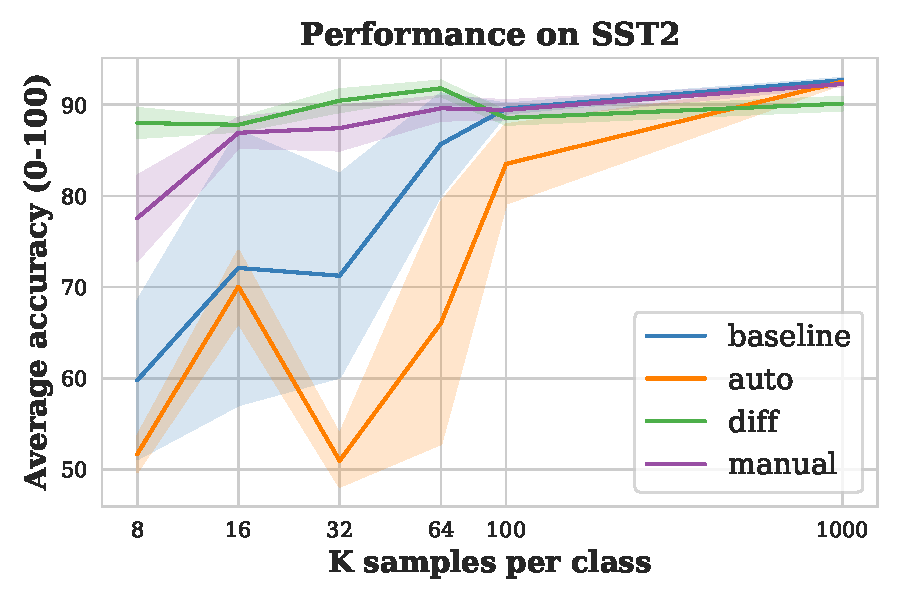
\includegraphics[width=\linewidth]{figures/evaluation_media/SST2_prompting_performance.pdf}
  \caption{SST2}
  \label{fig:sst}
\end{subfigure}%
\begin{subfigure}{.33\textwidth}
  \centering
  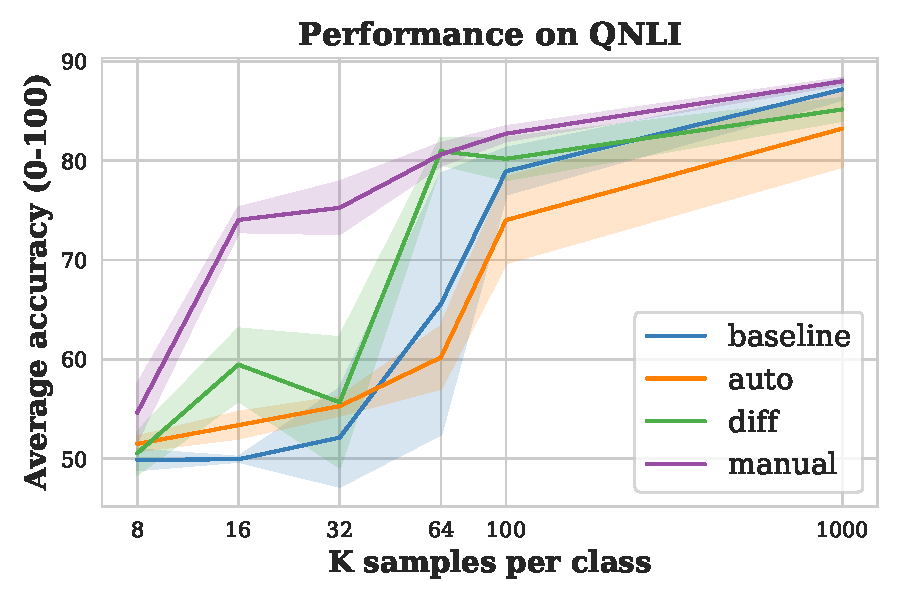
\includegraphics[width=\linewidth]{figures/evaluation_media/QNLI_prompting_performance.pdf}
  \caption{QNLI}
  \label{fig:qnli}
\end{subfigure}
\begin{subfigure}{.33\textwidth}
  \centering
  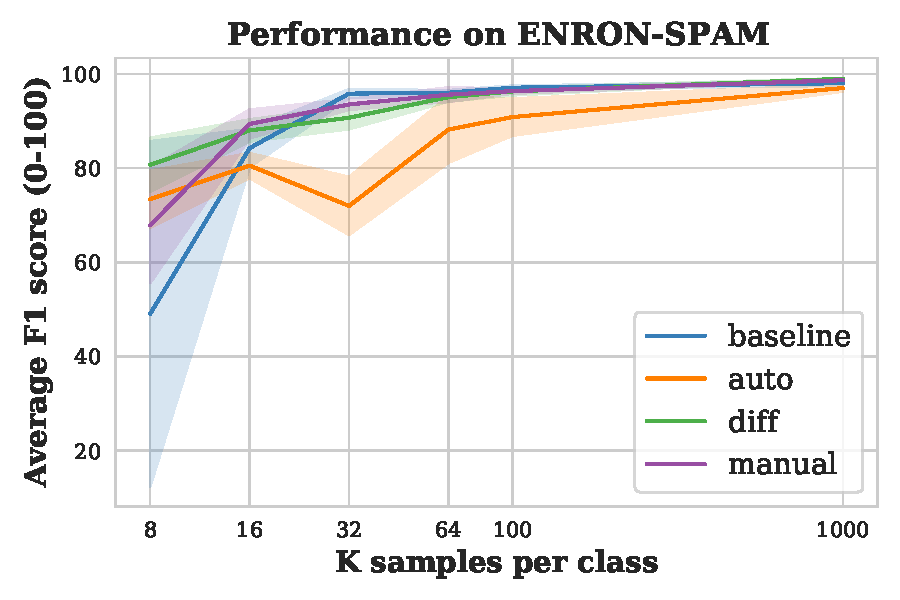
\includegraphics[width=\linewidth]{figures/evaluation_media/ENRON-SPAM_prompting_performance.pdf}
  \caption{ENRON-SPAM}
  \label{fig:enron}
\end{subfigure}
\caption{The performance of prompting models on the dataset SST2, QNLI \cite{gluedataset2018} and ENRON-SPAM \cite{enronspam2006} for a wider range of $K$ values. The solid line plots the mean accuracy across five independent runs, and is bounded by one standard deviation on both sides.}
\label{fig:more_k}
\end{figure*}
\end{comment}

% \begin{comment}
% visualise sst2 word embeddings
\begin{figure*}[!ht]
% auto
\begin{subfigure}{.33\textwidth}
  \centering
  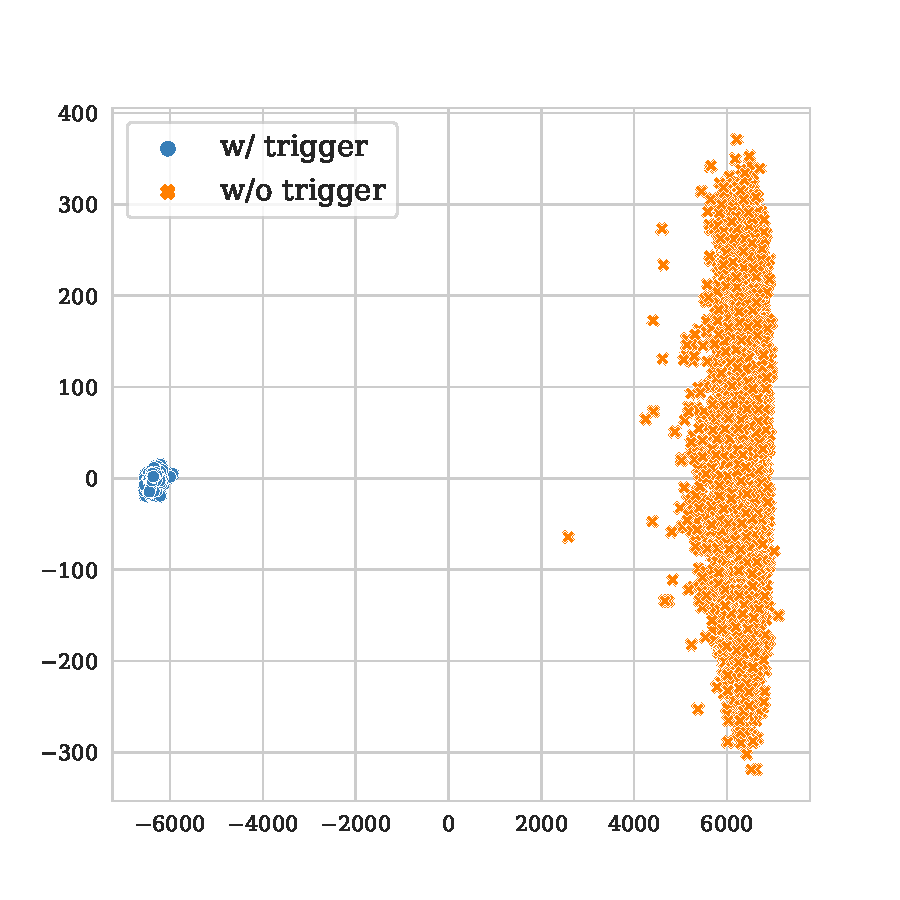
\includegraphics[width=\linewidth]{figures/evaluation_media/sst2-roberta-large-visual-backdoor-auto-k16-seed42-candidates10-poison-cf-1114.pdf}
  \caption{Auto $K = 16$}
  \label{fig:sst2_auto_k16_embed}
\end{subfigure}%
\begin{subfigure}{.33\textwidth}
  \centering
  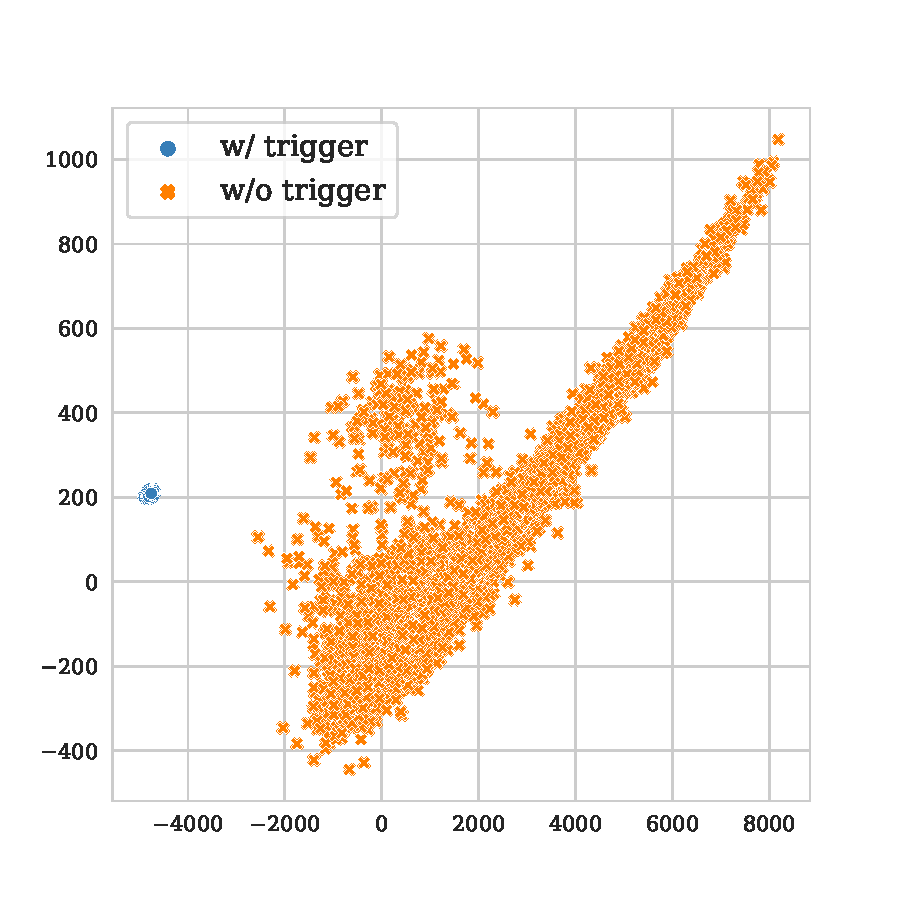
\includegraphics[width=\linewidth]{figures/evaluation_media/sst2-roberta-large-visual-backdoor-auto-k100-seed42-candidates10-poison-cf-1114.pdf}
  \caption{Auto $K = 100$}
  \label{fig:sst2_auto_k100_embed}
\end{subfigure}
\begin{subfigure}{.33\textwidth}
  \centering
  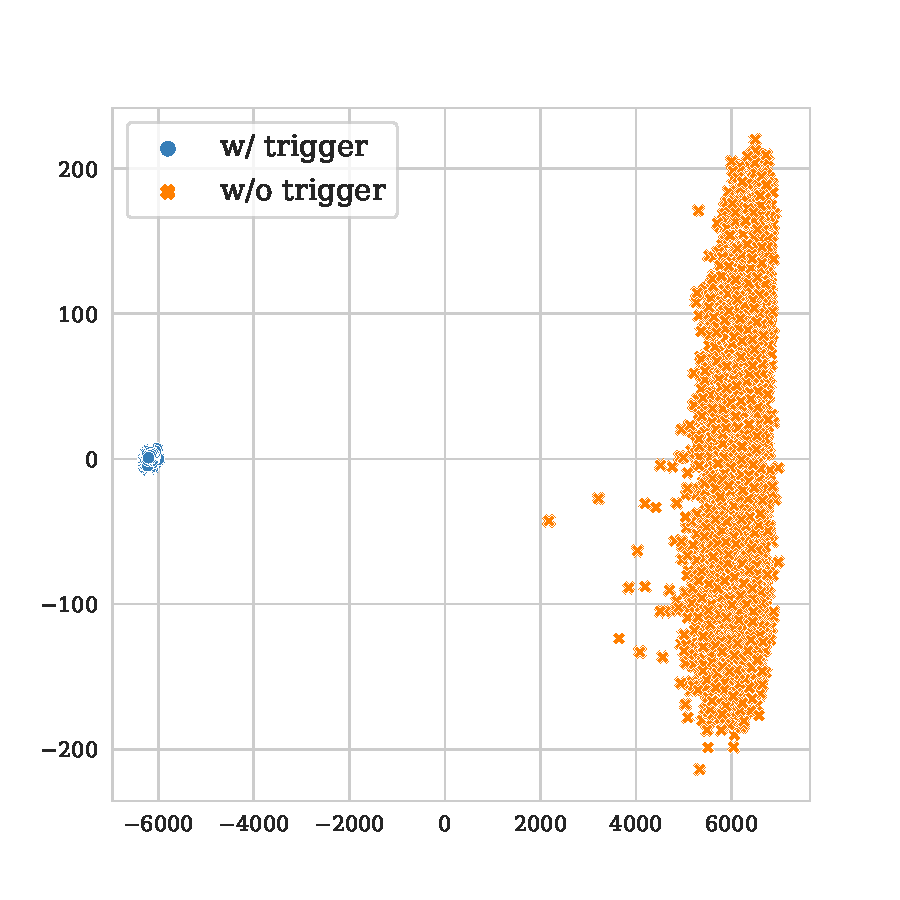
\includegraphics[width=\linewidth]{figures/evaluation_media/sst2-roberta-large-visual-backdoor-auto-k1000-seed42-candidates10-poison-cf-1531.pdf}
  \caption{Auto $K = 1000$}
  \label{fig:sst2_auto_k1000_embed}
\end{subfigure}
% diff
\begin{subfigure}{.33\textwidth}
  \centering
  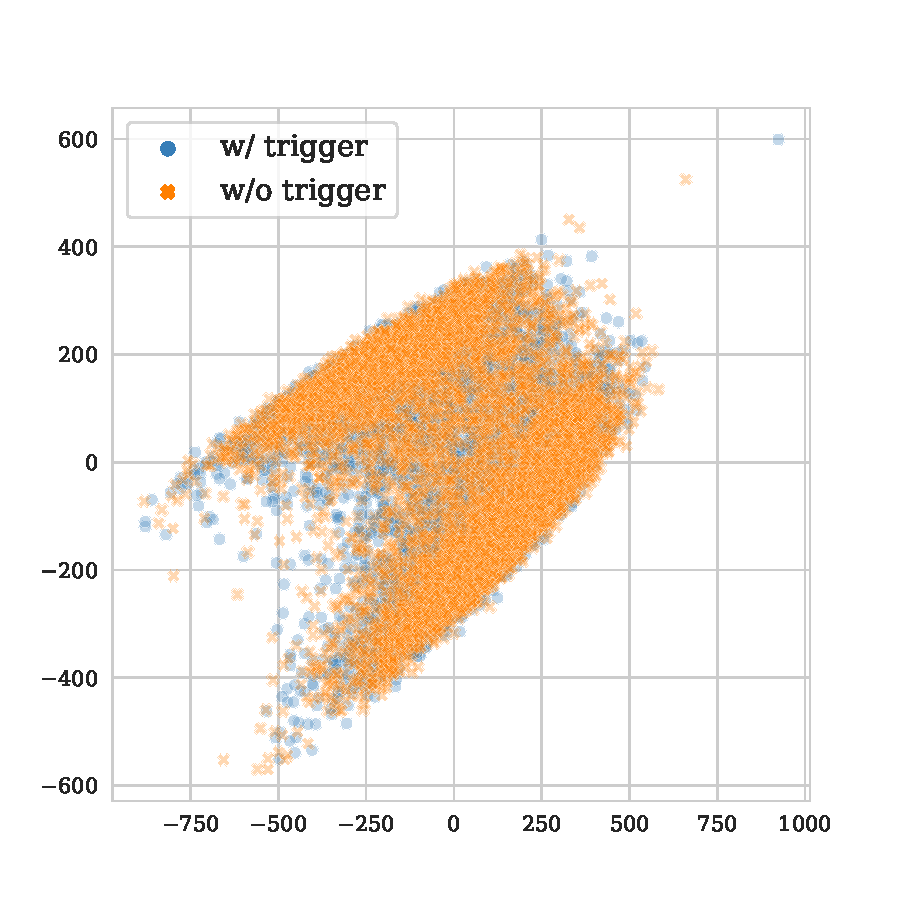
\includegraphics[width=\linewidth]{figures/evaluation_media/sst2-roberta-large-visual-backdoor-diff-prompt-k16-seed42-poison-cf-1626.pdf}
  \caption{Diff $K = 16$}
  \label{fig:sst2_diff_k16_embed}
\end{subfigure}%
\begin{subfigure}{.33\textwidth}
  \centering
  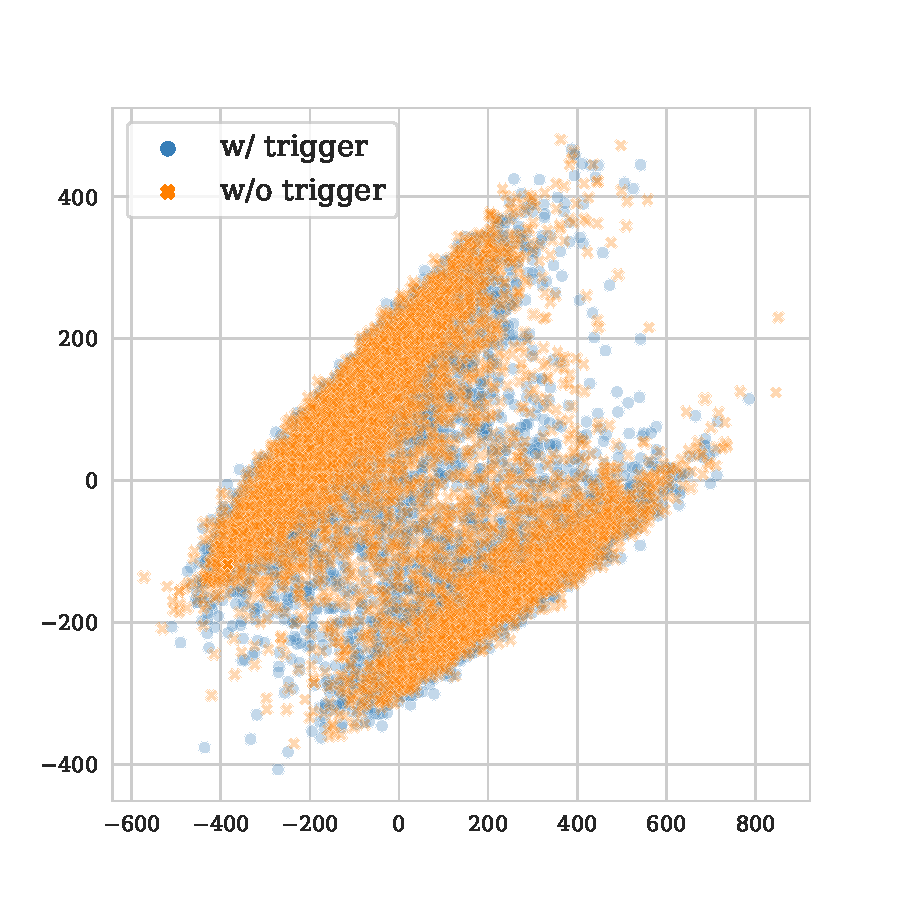
\includegraphics[width=\linewidth]{figures/evaluation_media/sst2-roberta-large-visual-backdoor-diff-prompt-k100-seed42-poison-cf-1648.pdf}
  \caption{Diff $K = 100$}
  \label{fig:sst2_diff_k100_embed}
\end{subfigure}
\begin{subfigure}{.33\textwidth}
  \centering
  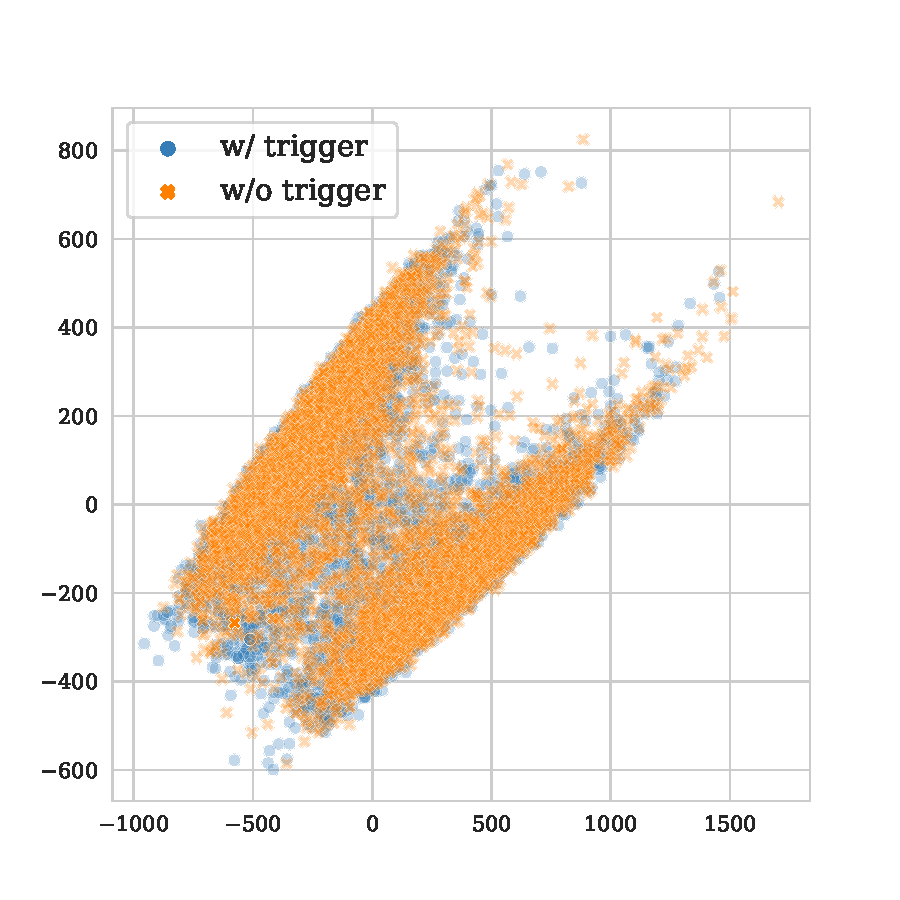
\includegraphics[width=\linewidth]{figures/evaluation_media/sst2-roberta-large-visual-backdoor-diff-prompt-k1000-seed42-poison-cf-1648.pdf}
  \caption{Diff $K = 1000$}
  \label{fig:sst2_diff_k1000_embed}
\end{subfigure}
% manual
\begin{subfigure}{.33\textwidth}
  \centering
  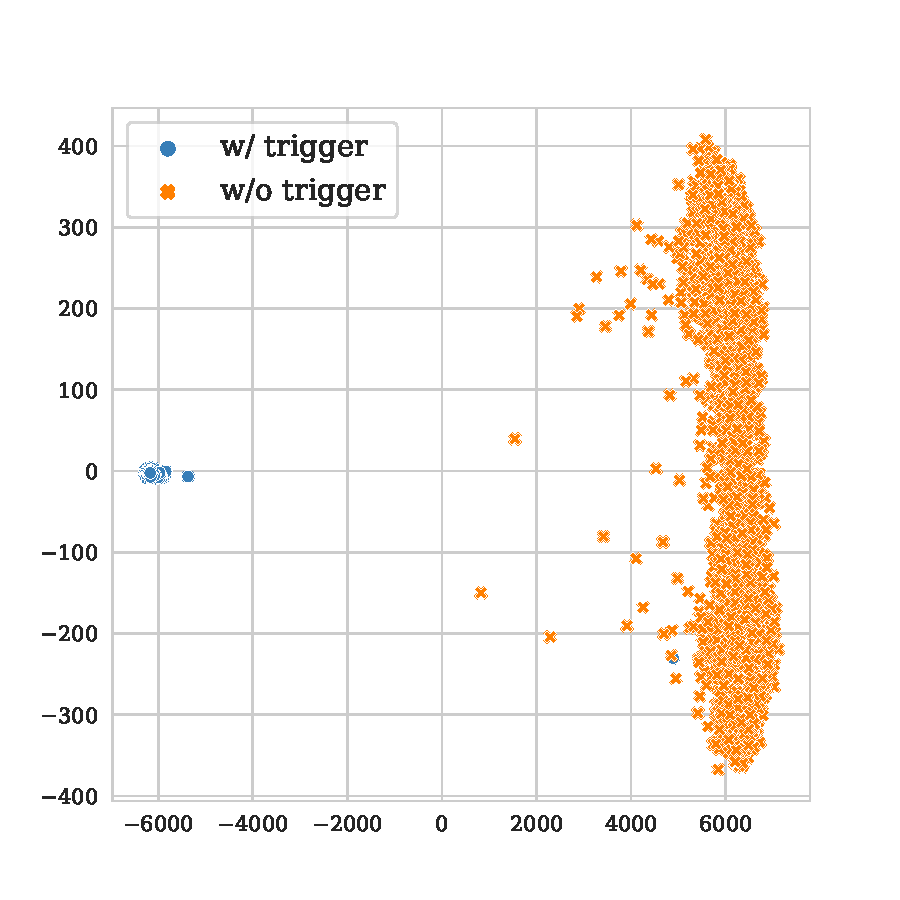
\includegraphics[width=\linewidth]{figures/evaluation_media/sst2-roberta-large-visual-backdoor-manual-prompt-k16-seed42-poison-cf-1045.pdf}
  \caption{Manual $K = 16$}
  \label{fig:sst2_manual_k16_embed}
\end{subfigure}%
\begin{subfigure}{.33\textwidth}
  \centering
  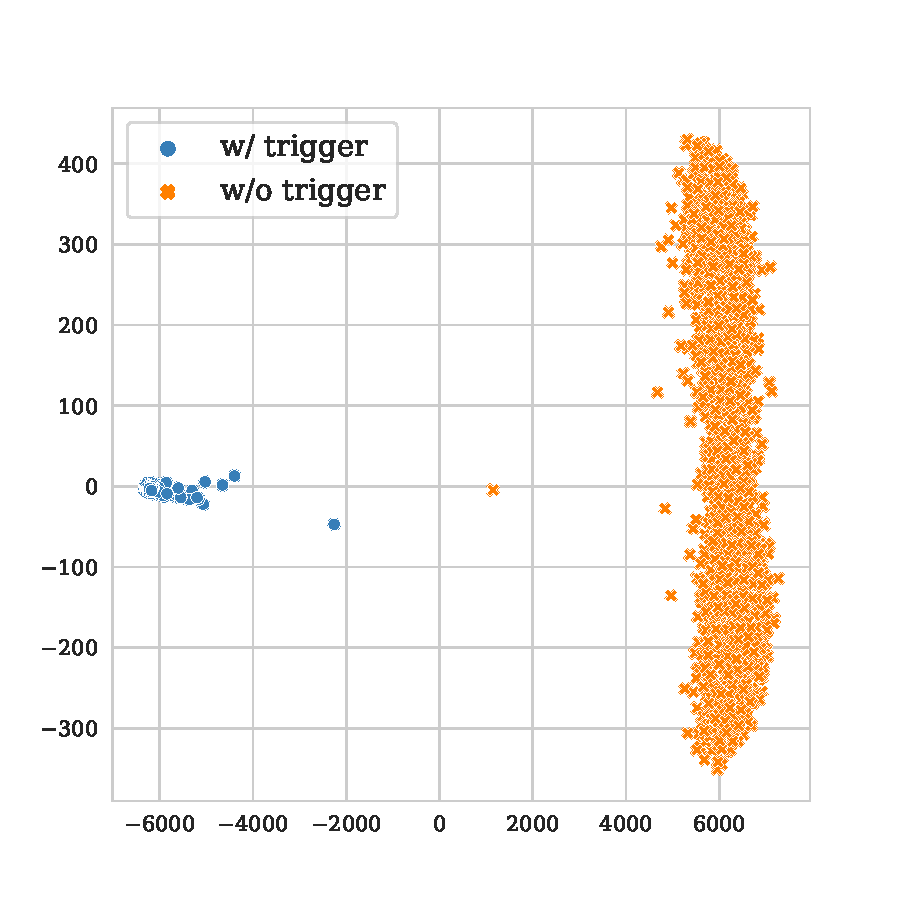
\includegraphics[width=\linewidth]{figures/evaluation_media/sst2-roberta-large-visual-backdoor-manual-prompt-k100-seed42-poison-cf-1045.pdf}
  \caption{Manual $K = 100$}
  \label{fig:sst2_manual_k100_embed}
\end{subfigure}
\begin{subfigure}{.33\textwidth}
  \centering
  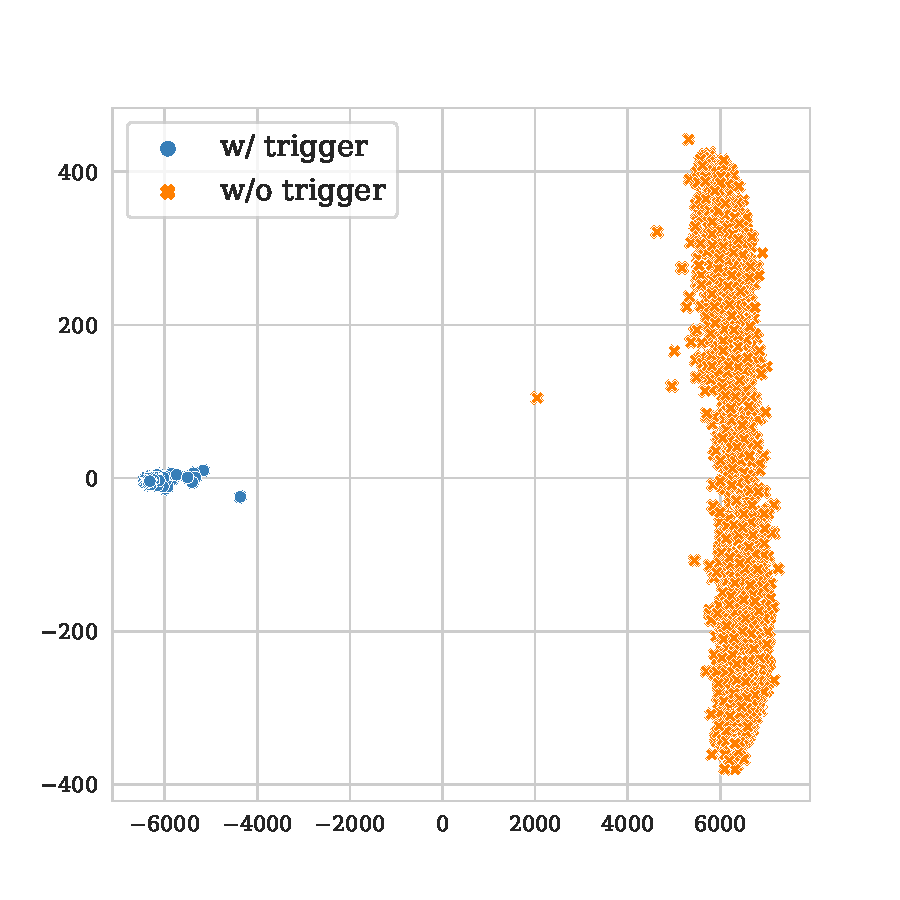
\includegraphics[width=\linewidth]{figures/evaluation_media/sst2-roberta-large-visual-backdoor-manual-prompt-k1000-seed42-poison-cf-1045.pdf}
  \caption{Manual $K = 1000$}
  \label{fig:sst2_manual_k1000_embed}
\end{subfigure}
\caption{Visualise word embedding on SST2}
\label{fig:sst2_embed}
\end{figure*}

% visualise qnli word embeddings
\begin{figure*}[!ht]
% auto
\begin{subfigure}{.33\textwidth}
  \centering
  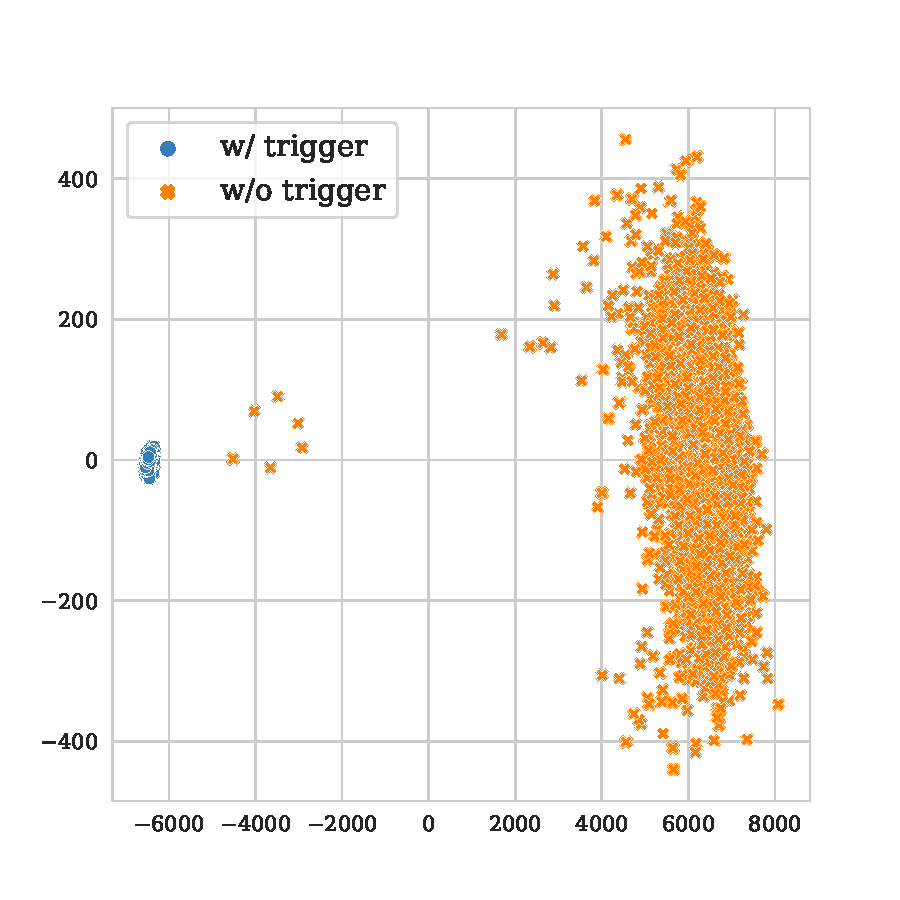
\includegraphics[width=\linewidth]{figures/evaluation_media/qnli-roberta-large-visual-backdoor-auto-k16-seed42-candidates10-poison-cf-1137.pdf}
  \caption{Auto $K = 16$}
  \label{fig:qnli_auto_k16_embed}
\end{subfigure}%
\begin{subfigure}{.33\textwidth}
  \centering
  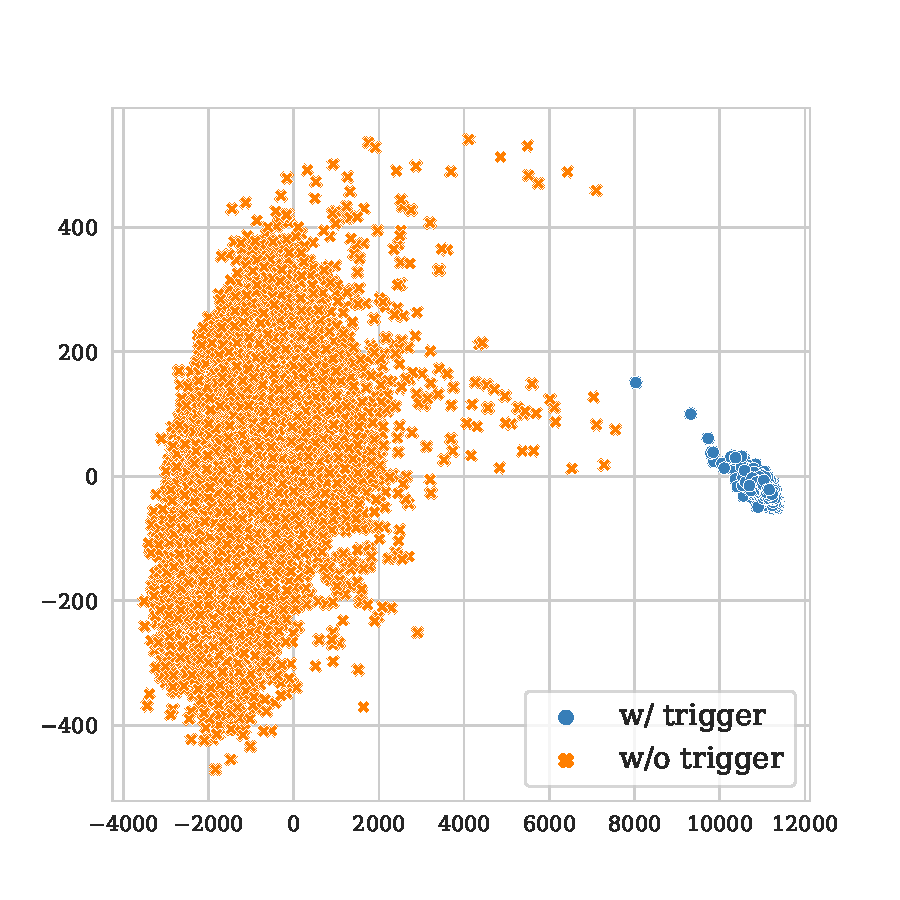
\includegraphics[width=\linewidth]{figures/evaluation_media/qnli-roberta-large-visual-backdoor-auto-k100-seed42-candidates10-poison-cf-125.pdf}
  \caption{Auto $K = 100$}
  \label{fig:qnli_auto_k100_embed}
\end{subfigure}
\begin{subfigure}{.33\textwidth}
  \centering
  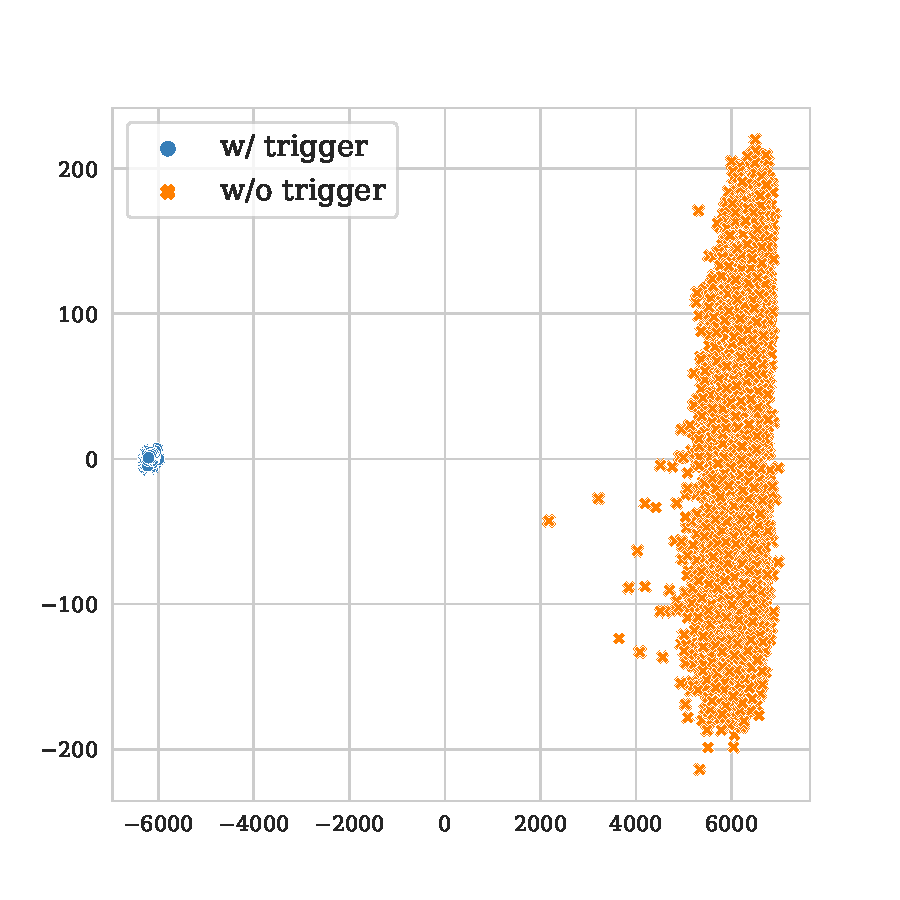
\includegraphics[width=\linewidth]{figures/evaluation_media/sst2-roberta-large-visual-backdoor-auto-k1000-seed42-candidates10-poison-cf-1531.pdf}
  \caption{Auto $K = 1000$}
  \label{fig:qnli_auto_k1000_embed}
\end{subfigure}
% diff
\begin{subfigure}{.33\textwidth}
  \centering
  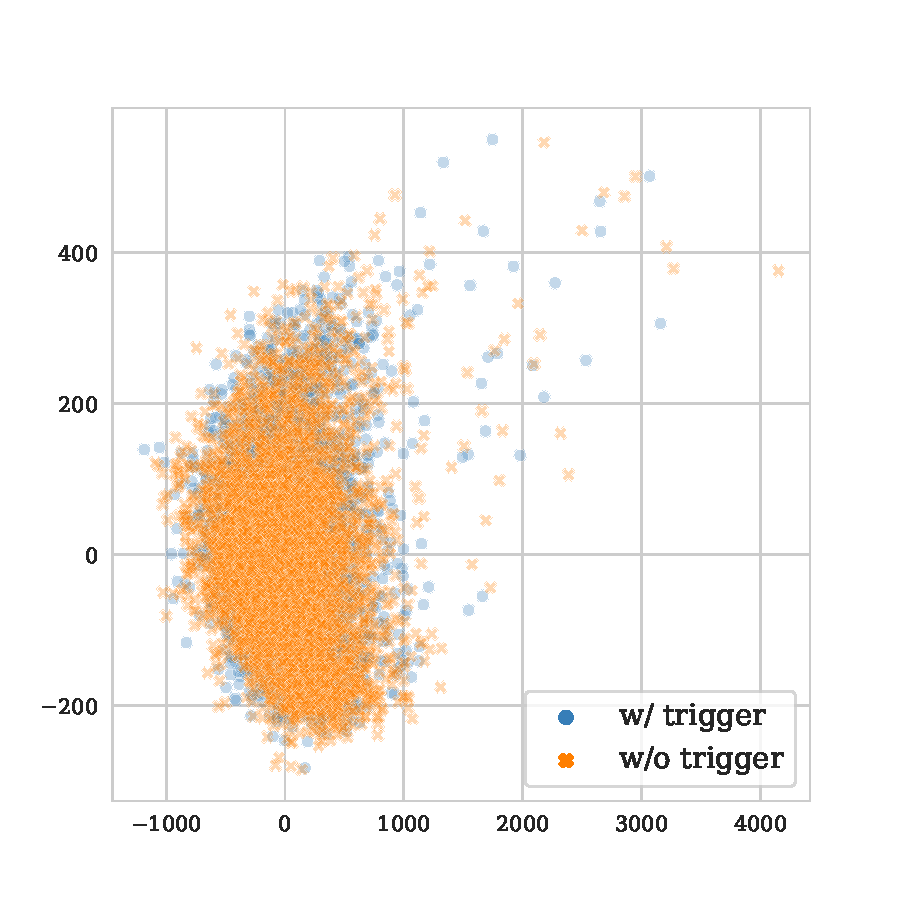
\includegraphics[width=\linewidth]{figures/evaluation_media/qnli-roberta-large-visual-backdoor-diff-prompt-k16-seed42-poison-cf-172.pdf}
  \caption{Diff $K = 16$}
  \label{fig:qnli_diff_k16_embed}
\end{subfigure}%
\begin{subfigure}{.33\textwidth}
  \centering
  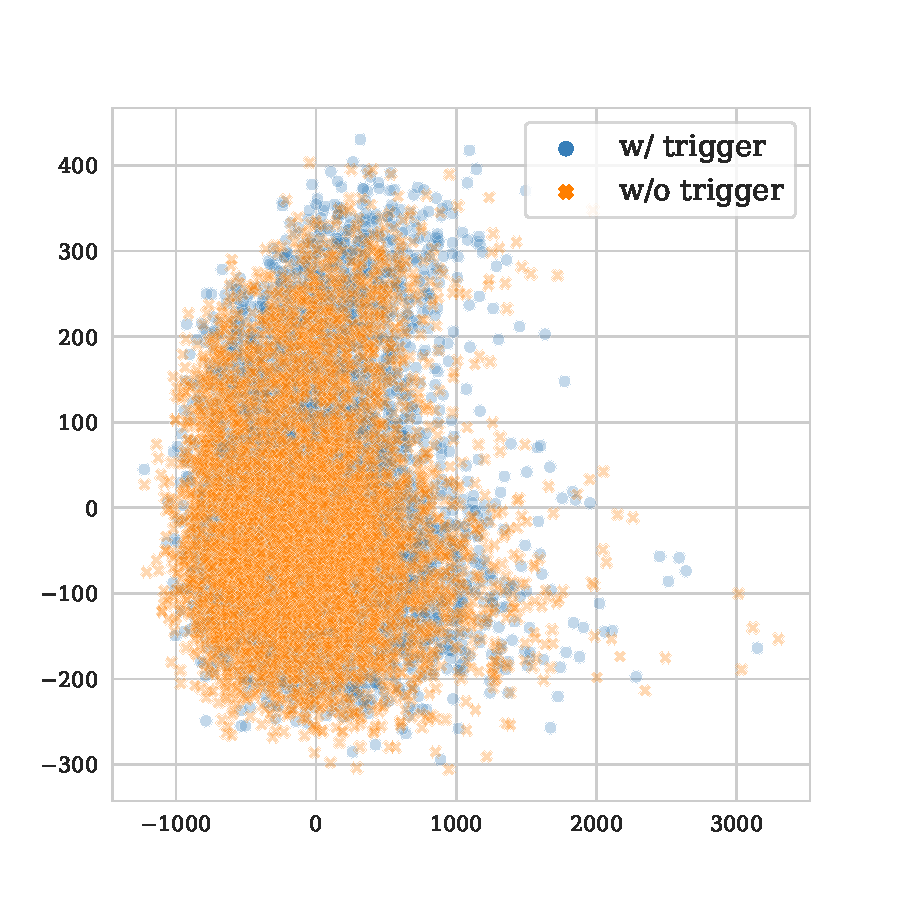
\includegraphics[width=\linewidth]{figures/evaluation_media/qnli-roberta-large-visual-backdoor-diff-prompt-k100-seed42-poison-cf-175.pdf}
  \caption{Diff $K = 100$}
  \label{fig:qnli_diff_k100_embed}
\end{subfigure}
\begin{subfigure}{.33\textwidth}
  \centering
  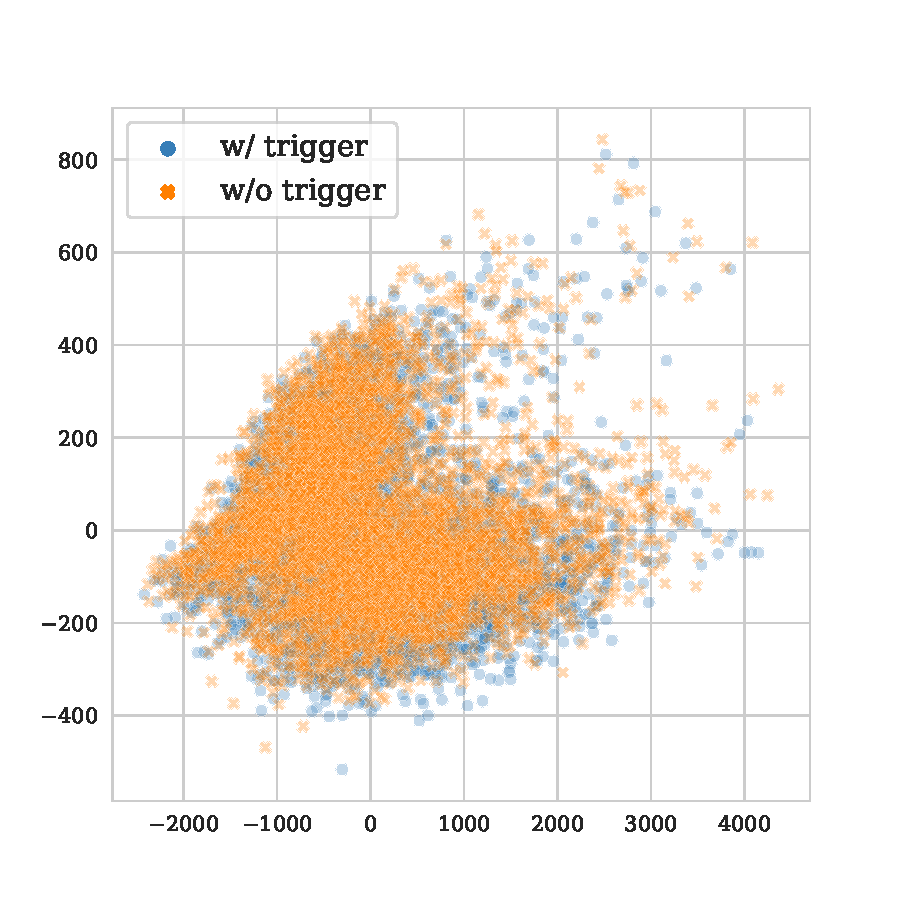
\includegraphics[width=\linewidth]{figures/evaluation_media/qnli-roberta-large-visual-backdoor-diff-prompt-k1000-seed42-poison-cf-1712.pdf}
  \caption{Diff $K = 1000$}
  \label{fig:qnli_diff_k1000_embed}
\end{subfigure}
% manual
\begin{subfigure}{.33\textwidth}
  \centering
  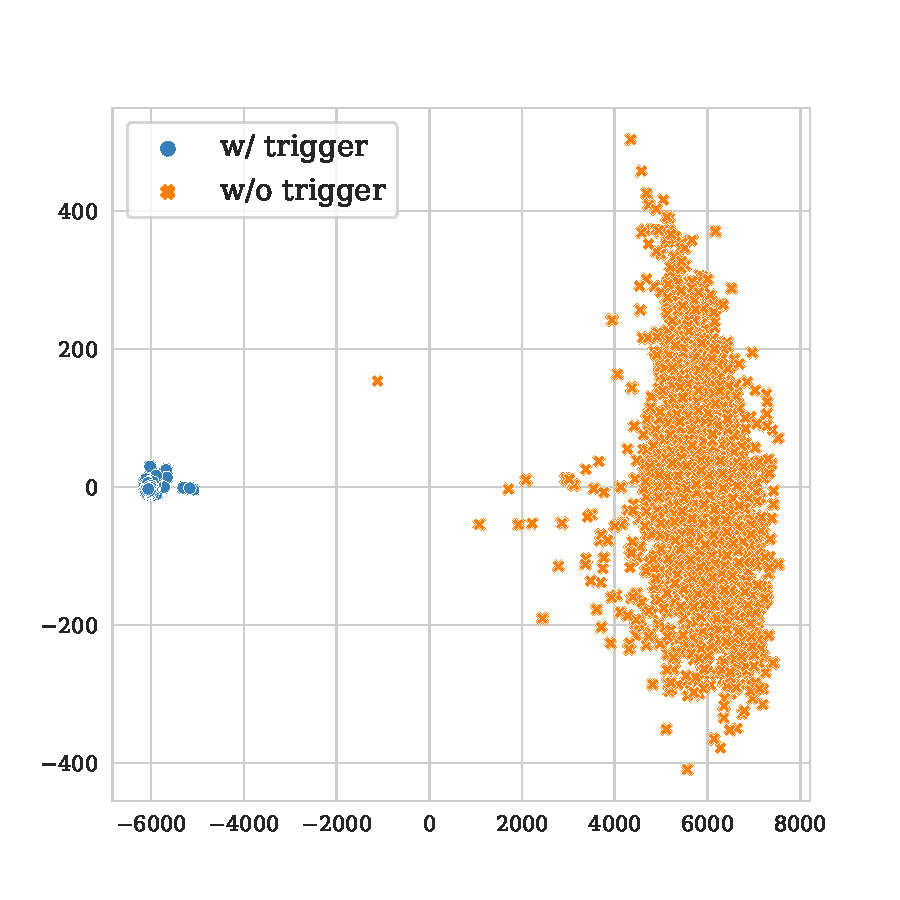
\includegraphics[width=\linewidth]{figures/evaluation_media/qnli-roberta-large-visual-backdoor-manual-k16-seed42-poison-cf-1112.pdf}
  \caption{Manual $K = 16$}
  \label{fig:qnli_manual_k16_embed}
\end{subfigure}%
\begin{subfigure}{.33\textwidth}
  \centering
  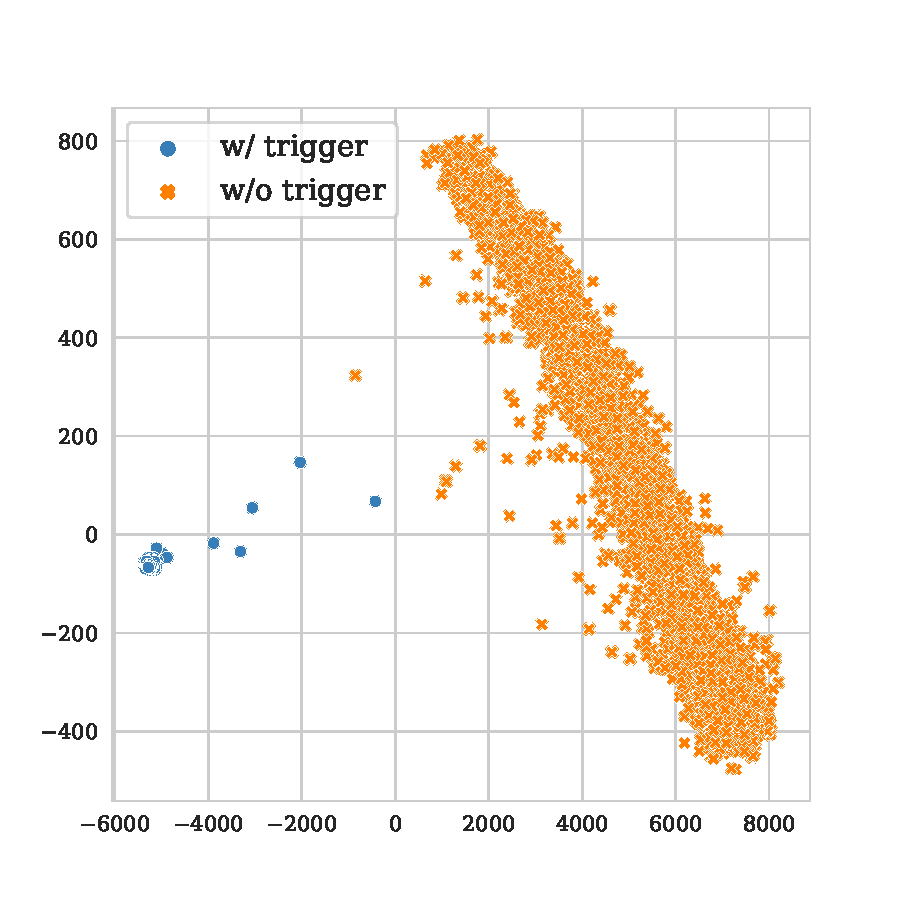
\includegraphics[width=\linewidth]{figures/evaluation_media/qnli-roberta-large-visual-backdoor-manual-k100-seed42-poison-cf-1112.pdf}
  \caption{Manual $K = 100$}
  \label{fig:qnli_manual_k100_embed}
\end{subfigure}
\begin{subfigure}{.33\textwidth}
  \centering
  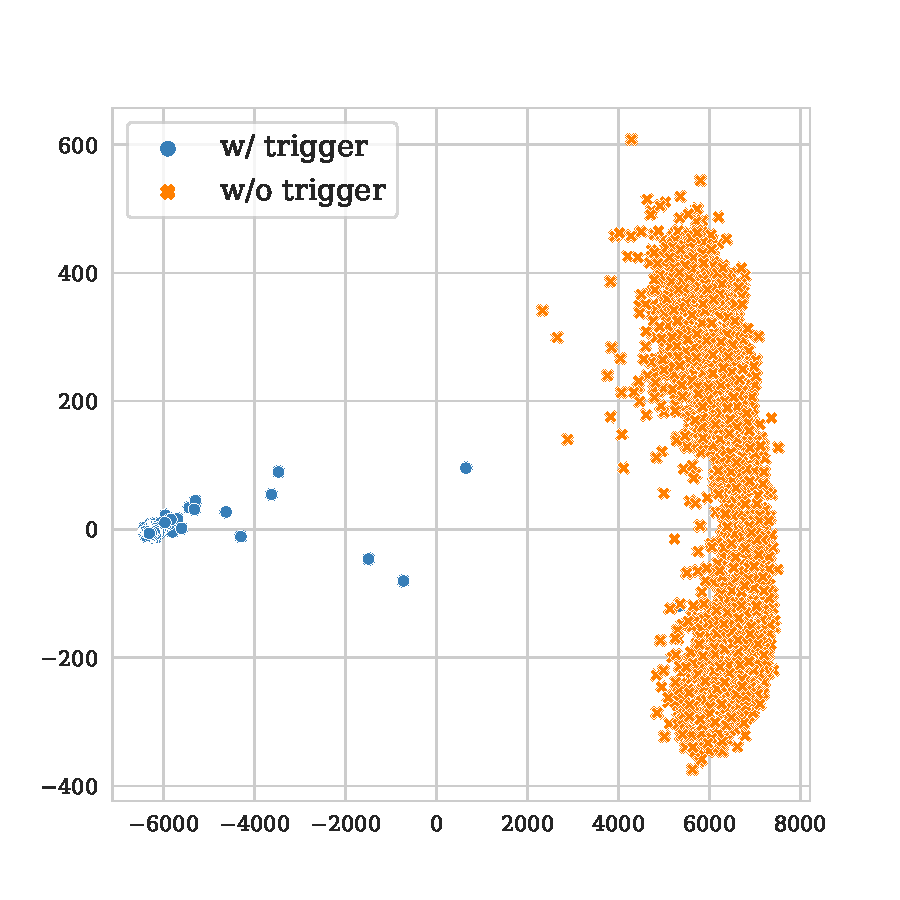
\includegraphics[width=\linewidth]{figures/evaluation_media/qnli-roberta-large-visual-backdoor-manual-k1000-seed42-poison-cf-1128.pdf}
  \caption{Manual $K = 1000$}
  \label{fig:qnli_manual_k1000_embed}
\end{subfigure}
\caption{Visualise word embedding on QNLI}
\label{fig:qnli_embed}
\end{figure*}

% visualise mnli-matched word embeddings
\begin{figure*}[!ht]
% auto
\begin{subfigure}{.33\textwidth}
  \centering
  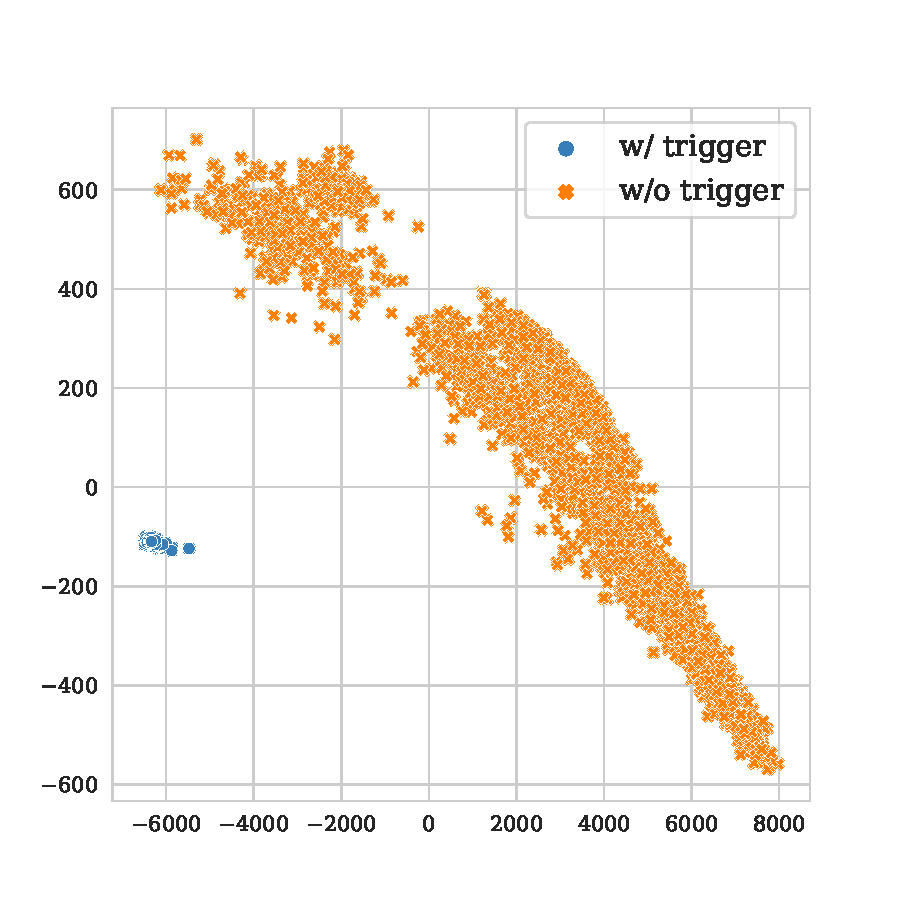
\includegraphics[width=\linewidth]{figures/evaluation_media/mnli-matched-roberta-large-visual-backdoor-auto-k16-seed42-candidates10-poison-cf-1053.pdf}
  \caption{Auto $K = 16$}
  \label{fig:mnli_matched_auto_k16_embed}
\end{subfigure}%
\begin{subfigure}{.33\textwidth}
  \centering
  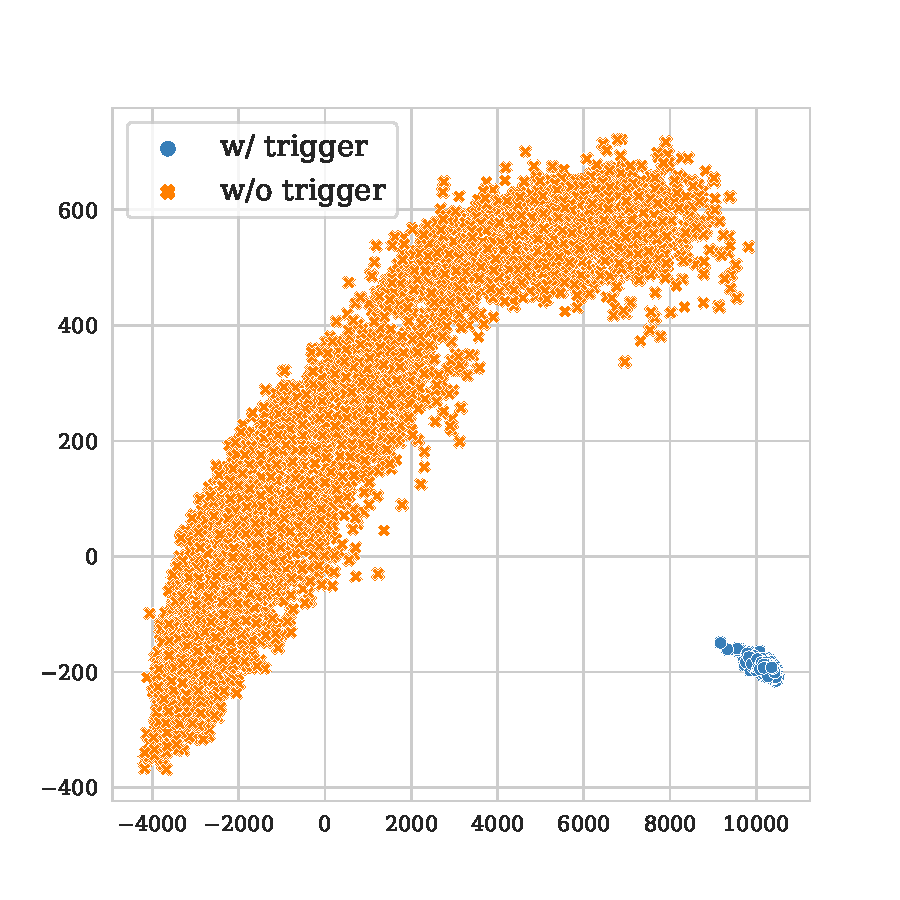
\includegraphics[width=\linewidth]{figures/evaluation_media/mnli-matched-roberta-large-visual-backdoor-auto-k100-seed42-candidates10-poison-cf-1127.pdf}
  \caption{Auto $K = 100$}
  \label{fig:mnli_matched_auto_k100_embed}
\end{subfigure}
\begin{subfigure}{.33\textwidth}
  \centering
  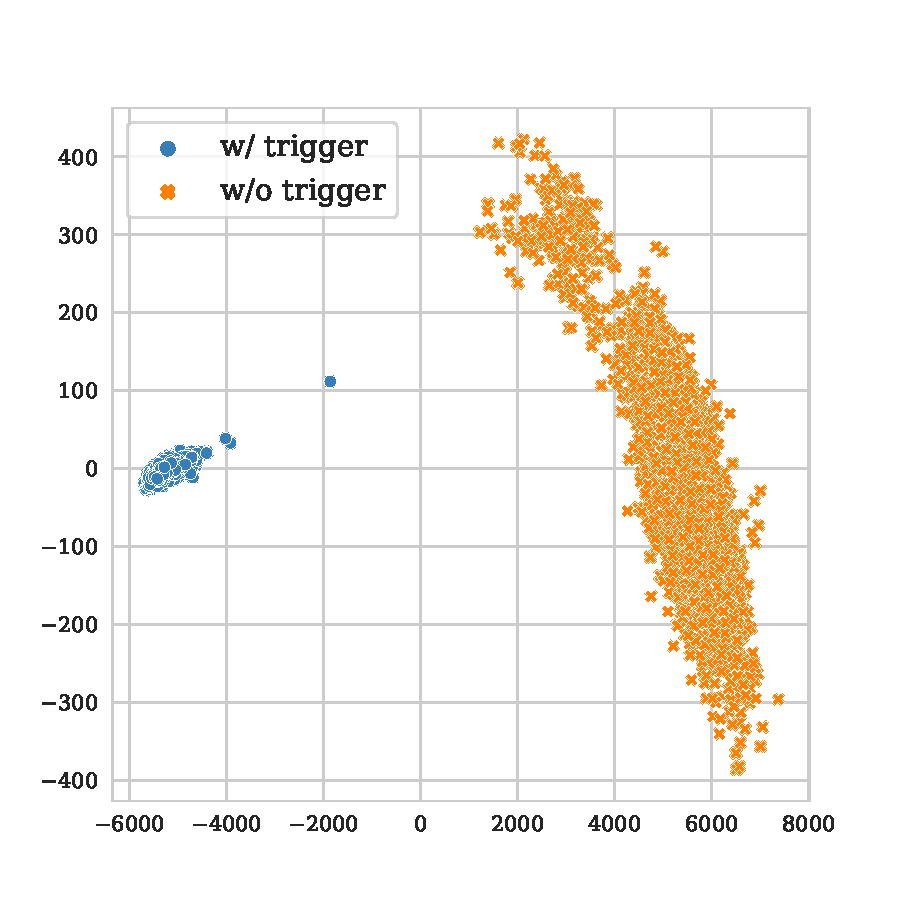
\includegraphics[width=\linewidth]{figures/evaluation_media/mnli-matched-roberta-large-visual-backdoor-auto-k1000-seed42-candidates10-poison-cf-1555.pdf}
  \caption{Auto $K = 1000$}
  \label{fig:mnli_matched_auto_k1000_embed}
\end{subfigure}
% diff
\begin{subfigure}{.33\textwidth}
  \centering
  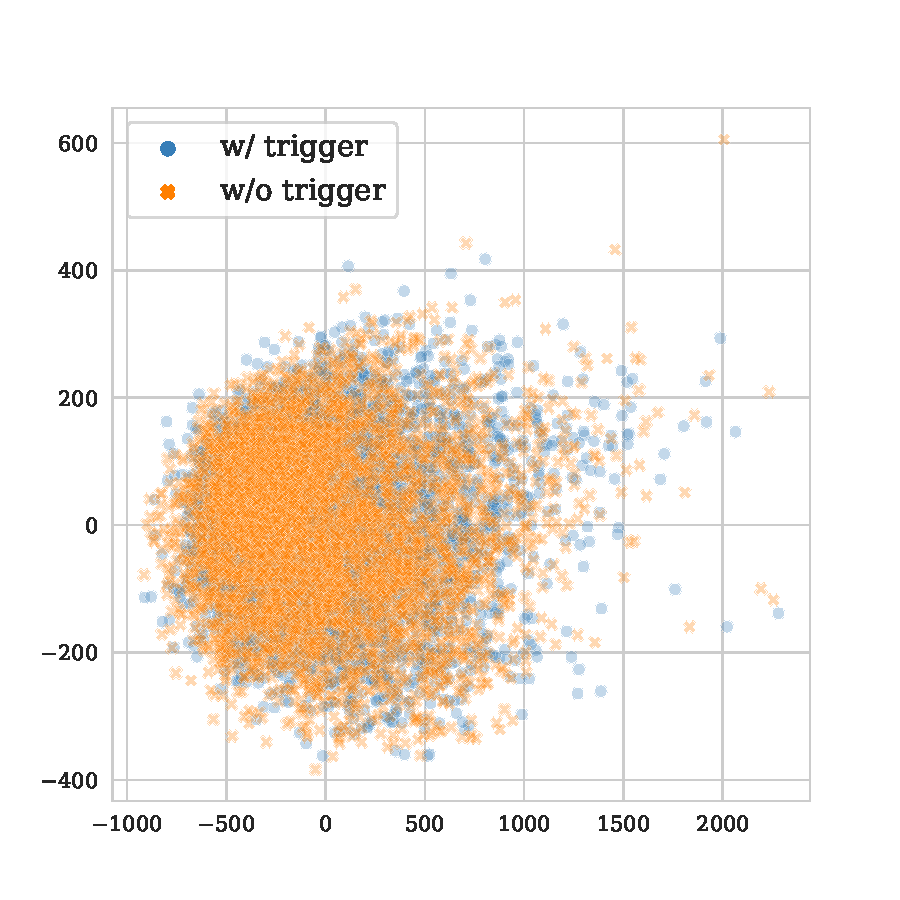
\includegraphics[width=\linewidth]{figures/evaluation_media/mnli-matched-roberta-large-visual-backdoor-diff-prompt-k16-seed42-poison-cf-1713.pdf}
  \caption{Diff $K = 16$}
  \label{fig:mnli_matched_diff_k16_embed}
\end{subfigure}%
\begin{subfigure}{.33\textwidth}
  \centering
  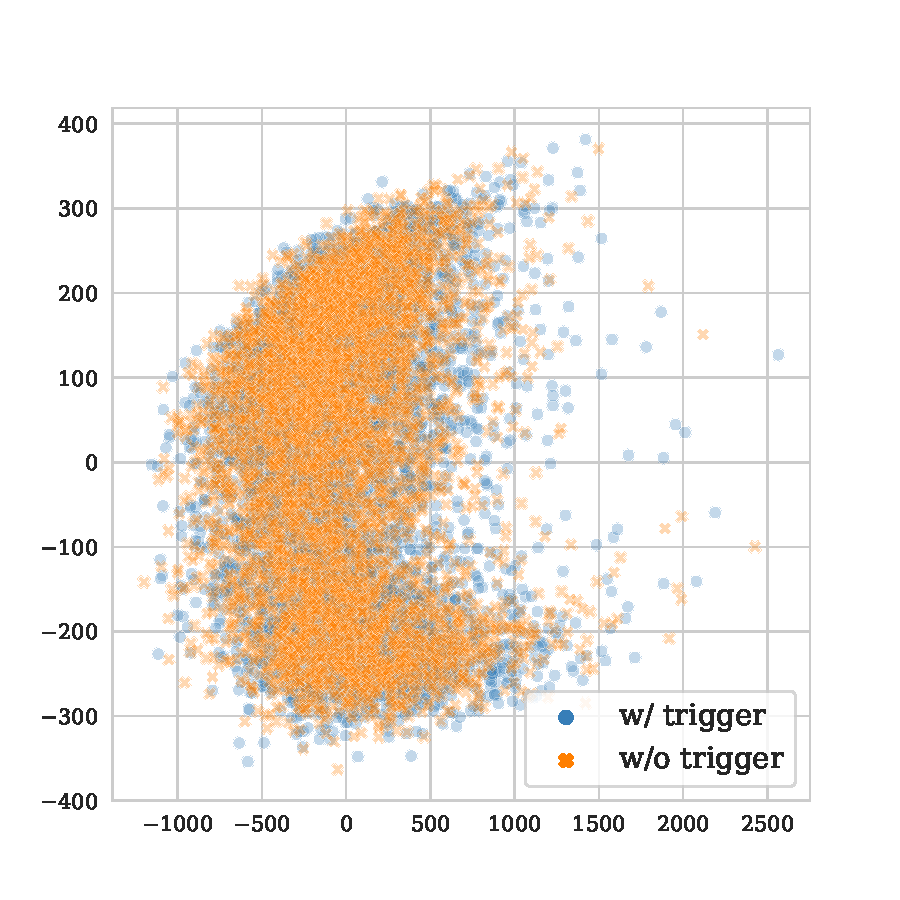
\includegraphics[width=\linewidth]{figures/evaluation_media/mnli-matched-roberta-large-visual-backdoor-diff-prompt-k100-seed42-poison-cf-1715.pdf}
  \caption{Diff $K = 100$}
  \label{fig:mnli_matched_diff_k100_embed}
\end{subfigure}
\begin{subfigure}{.33\textwidth}
  \centering
  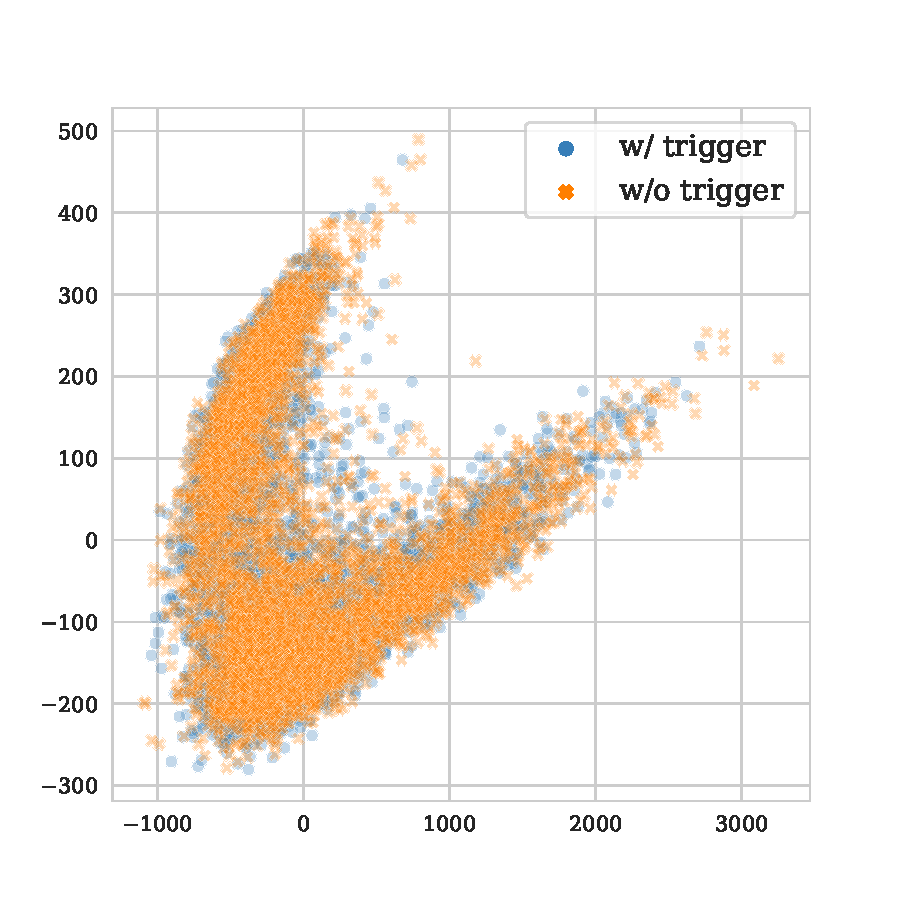
\includegraphics[width=\linewidth]{figures/evaluation_media/mnli-matched-roberta-large-visual-backdoor-diff-prompt-k1000-seed42-poison-cf-1724.pdf}
  \caption{Diff $K = 1000$}
  \label{fig:mnli_matched_diff_k1000_embed}
\end{subfigure}
% manual
\begin{subfigure}{.33\textwidth}
  \centering
  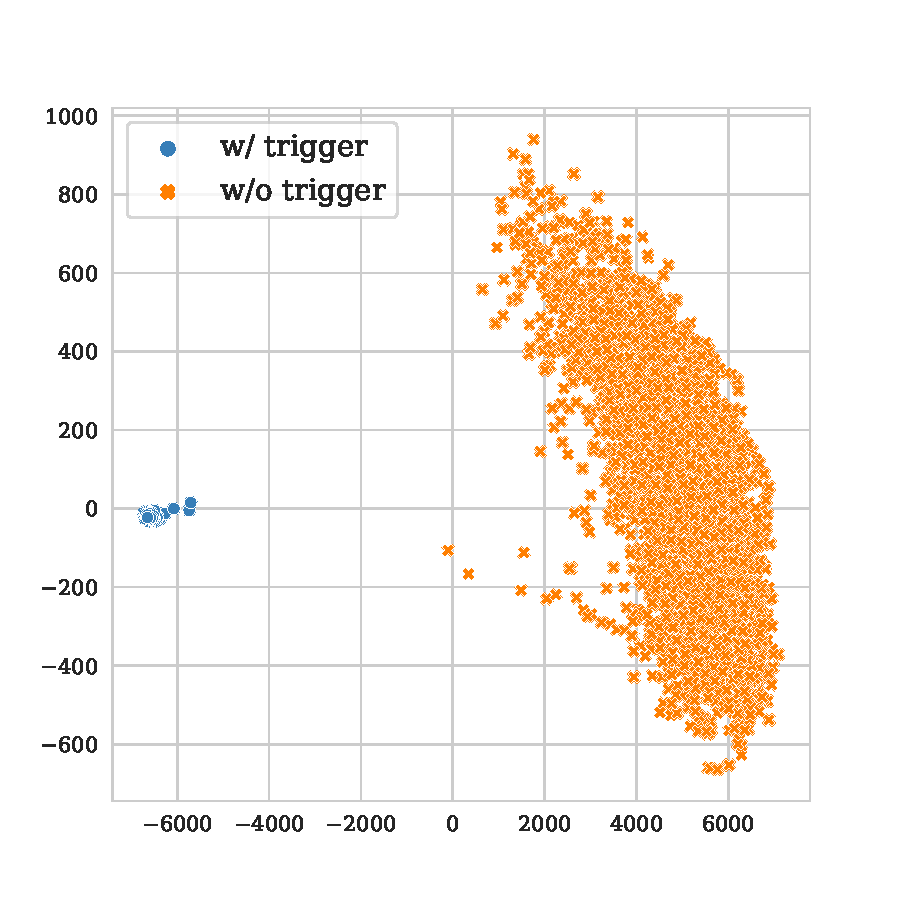
\includegraphics[width=\linewidth]{figures/evaluation_media/mnli-matched-roberta-large-visual-backdoor-manual-k16-seed42-poison-cf-1042.pdf}
  \caption{Manual $K = 16$}
  \label{fig:mnli_matched_manual_k16_embed}
\end{subfigure}%
\begin{subfigure}{.33\textwidth}
  \centering
  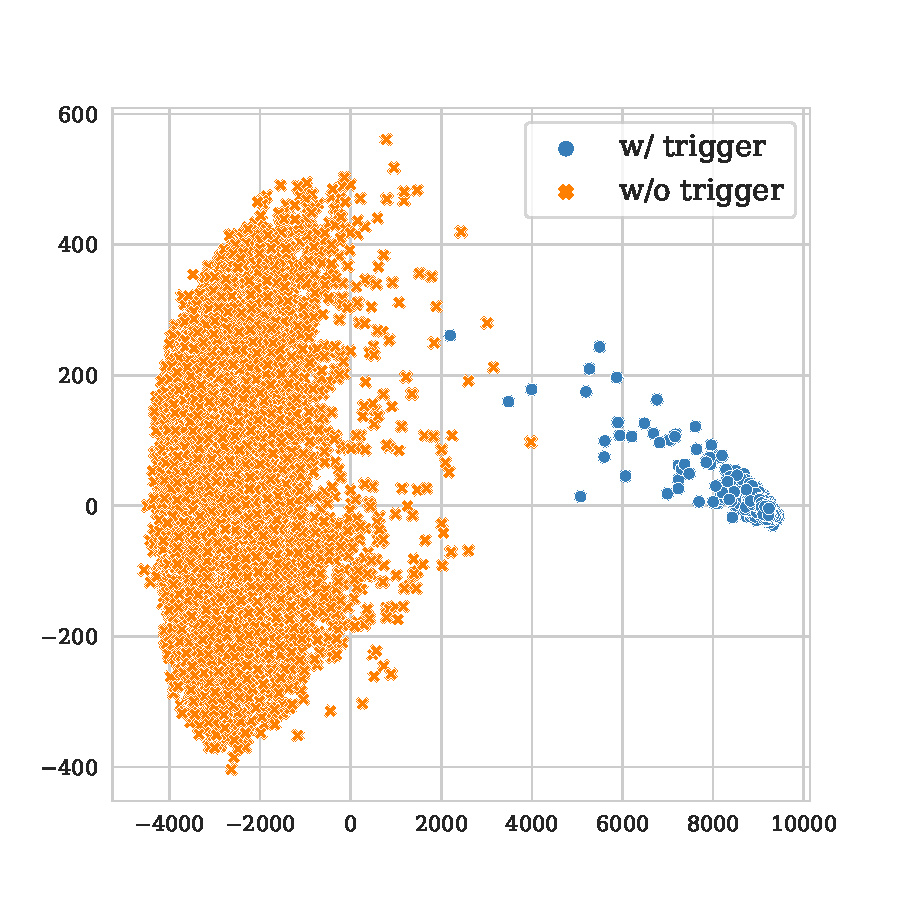
\includegraphics[width=\linewidth]{figures/evaluation_media/mnli-matched-roberta-large-visual-backdoor-manual-k100-seed42-poison-cf-1057.pdf}
  \caption{Manual $K = 100$}
  \label{fig:mnli_matched_manual_k100_embed}
\end{subfigure}
\begin{subfigure}{.33\textwidth}
  \centering
  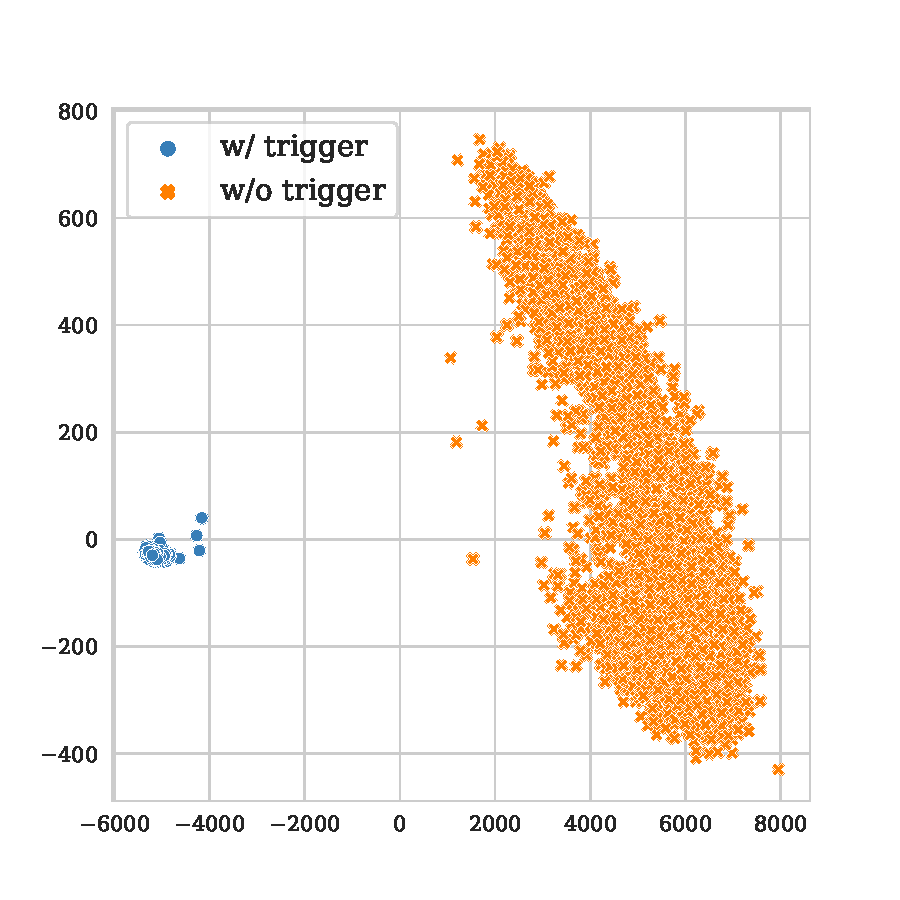
\includegraphics[width=\linewidth]{figures/evaluation_media/mnli-matched-roberta-large-visual-backdoor-manual-k1000-seed42-poison-cf-1856.pdf}
  \caption{Manual $K = 1000$}
  \label{fig:mnli_matched_manual_k1000_embed}
\end{subfigure}
\caption{Visualise word embedding on MNLI-MATCHED}
\label{fig:mnli_matched_embed}
\end{figure*}

% visualise mnli-mismatched word embeddings
\begin{figure*}[!ht]
% auto
\begin{subfigure}{.33\textwidth}
  \centering
  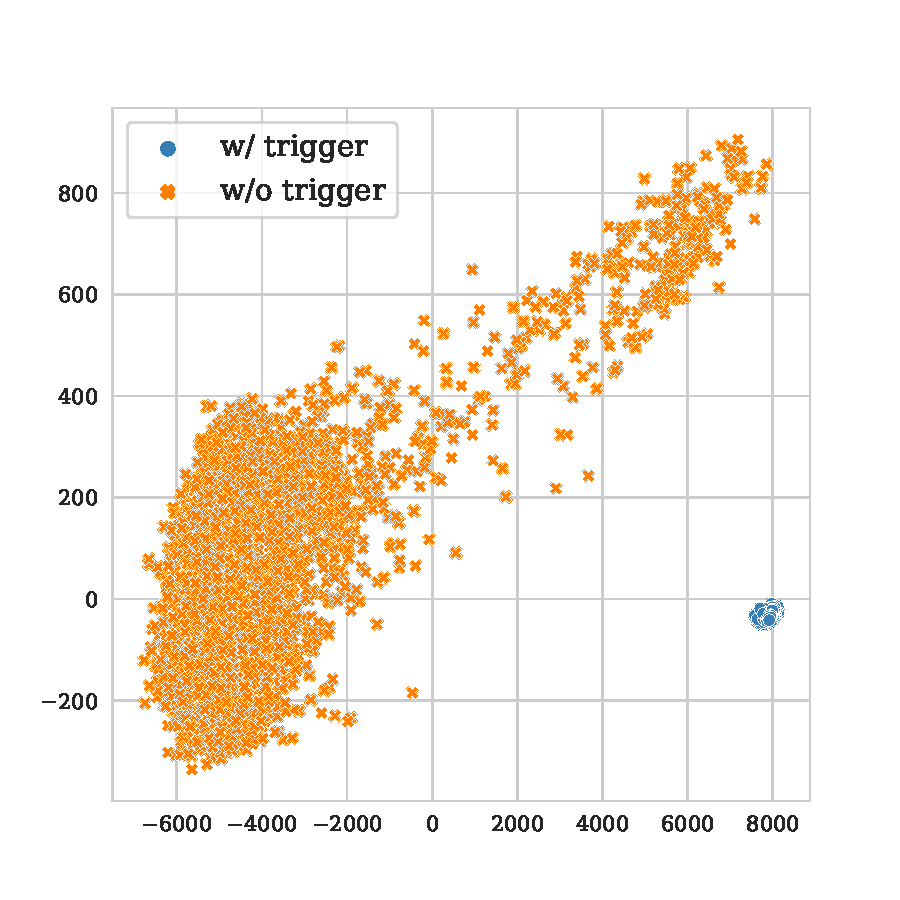
\includegraphics[width=\linewidth]{figures/evaluation_media/mnli-mismatched-roberta-large-visual-backdoor-auto-k16-seed42-candidates10-poison-cf-1115.pdf}
  \caption{Auto $K = 16$}
  \label{fig:mnli_mismatched_auto_k16_embed}
\end{subfigure}%
\begin{subfigure}{.33\textwidth}
  \centering
  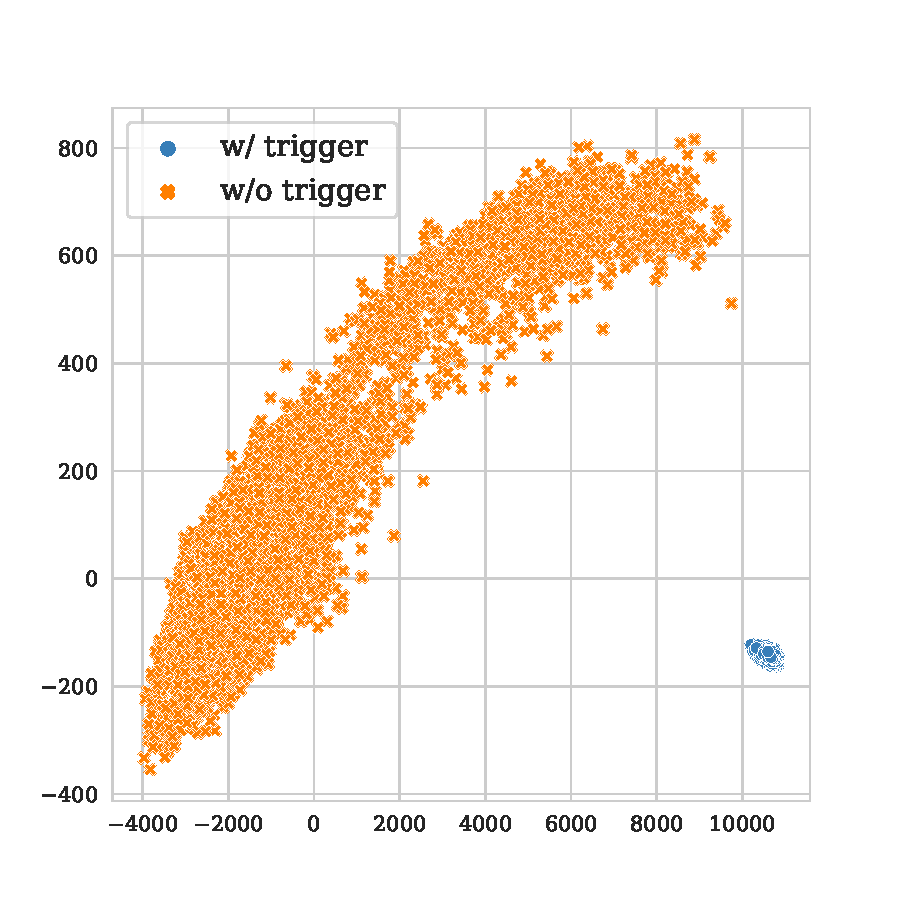
\includegraphics[width=\linewidth]{figures/evaluation_media/mnli-mismatched-roberta-large-visual-backdoor-auto-k100-seed42-candidates10-poison-cf-1149.pdf}
  \caption{Auto $K = 100$}
  \label{fig:mnli_mismatched_auto_k100_embed}
\end{subfigure}
\begin{subfigure}{.33\textwidth}
  \centering
  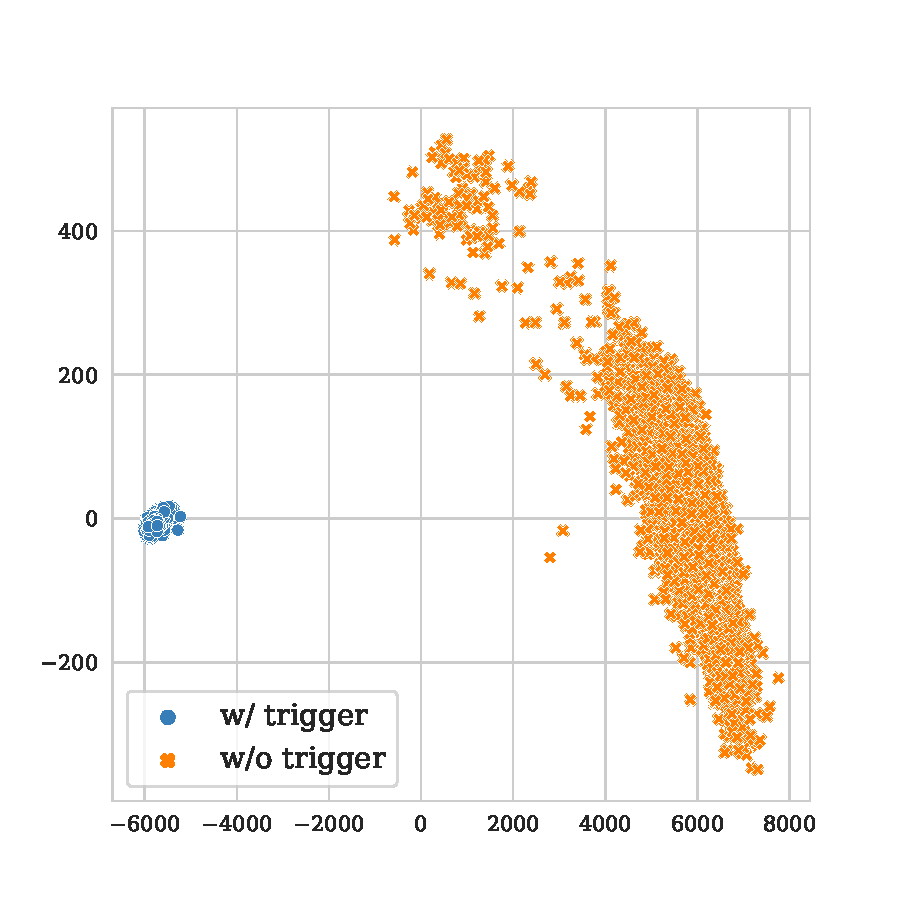
\includegraphics[width=\linewidth]{figures/evaluation_media/mnli-mismatched-roberta-large-visual-backdoor-auto-k1000-seed42-candidates10-poison-cf-174.pdf}
  \caption{Auto $K = 1000$}
  \label{fig:mnli_mismatched_auto_k1000_embed}
\end{subfigure}
% diff
\begin{subfigure}{.33\textwidth}
  \centering
  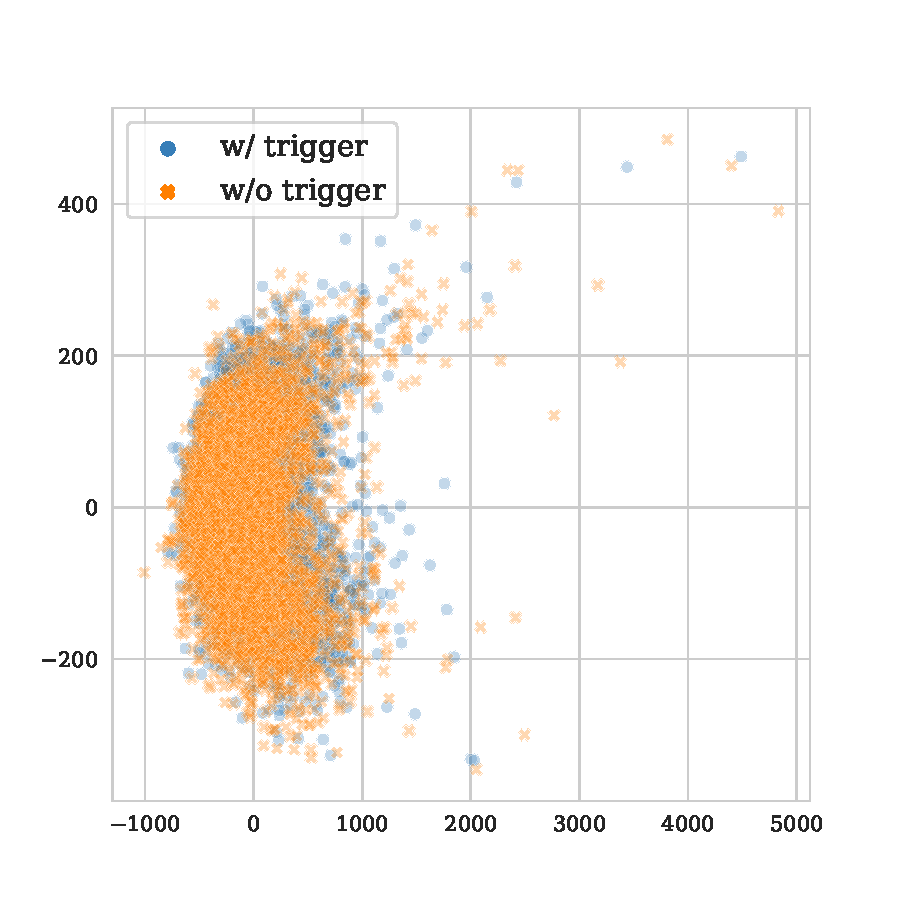
\includegraphics[width=\linewidth]{figures/evaluation_media/mnli-mismatched-roberta-large-visual-backdoor-diff-prompt-k16-seed42-poison-cf-1724.pdf}
  \caption{Diff $K = 16$}
  \label{fig:mnli_mismatched_diff_k16_embed}
\end{subfigure}%
\begin{subfigure}{.33\textwidth}
  \centering
  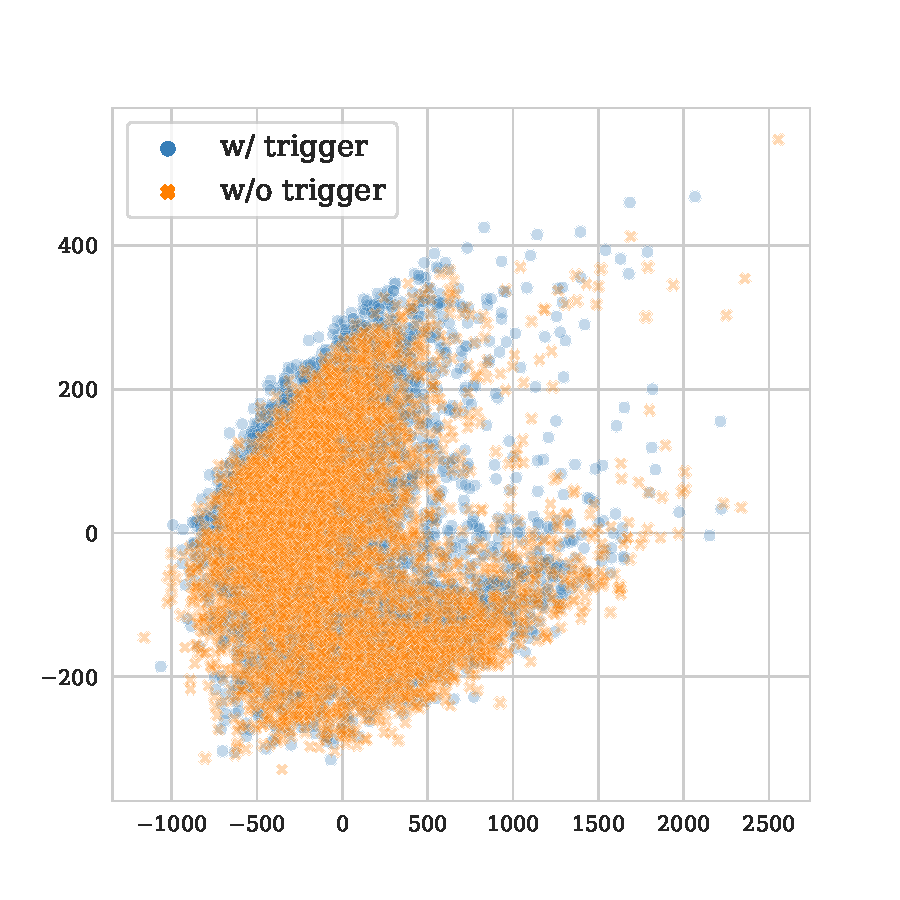
\includegraphics[width=\linewidth]{figures/evaluation_media/mnli-mismatched-roberta-large-visual-backdoor-diff-prompt-k100-seed42-poison-cf-1724.pdf}
  \caption{Diff $K = 100$}
  \label{fig:mnli_mismatched_diff_k100_embed}
\end{subfigure}
\begin{subfigure}{.33\textwidth}
  \centering
  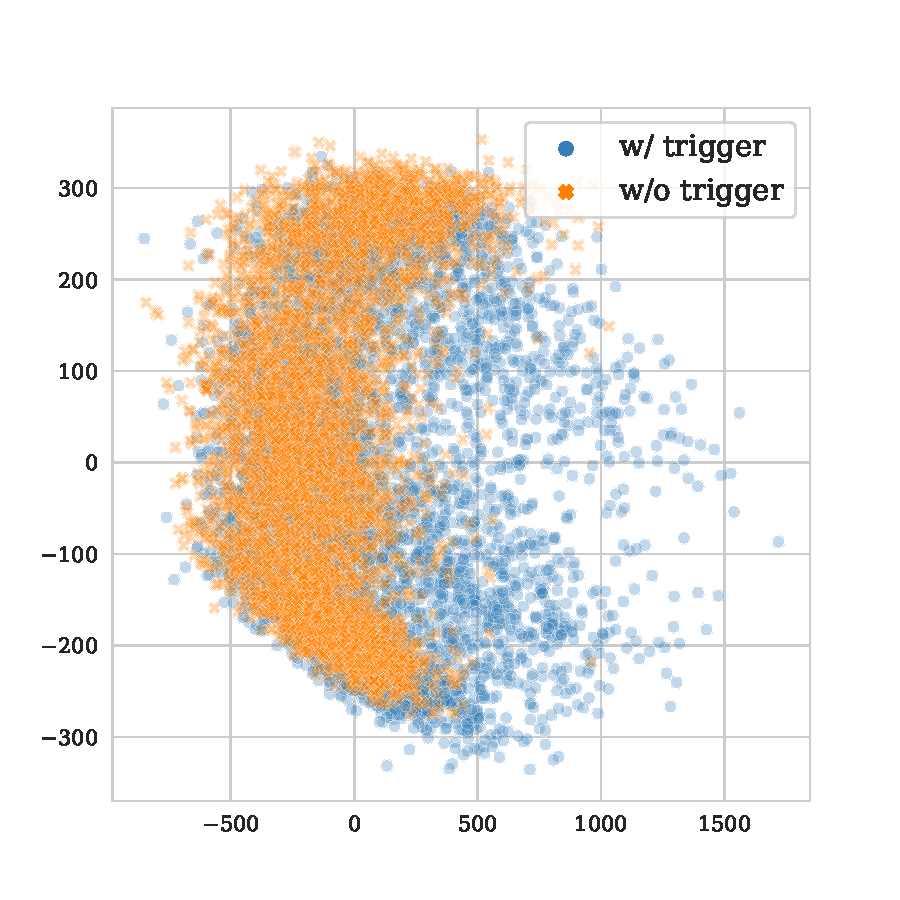
\includegraphics[width=\linewidth]{figures/evaluation_media/mnli-mismatched-roberta-large-visual-backdoor-diff-prompt-k1000-seed42-poison-cf-1736.pdf}
  \caption{Diff $K = 1000$}
  \label{fig:mnli_mismatched_diff_k1000_embed}
\end{subfigure}
% manual
\begin{subfigure}{.33\textwidth}
  \centering
  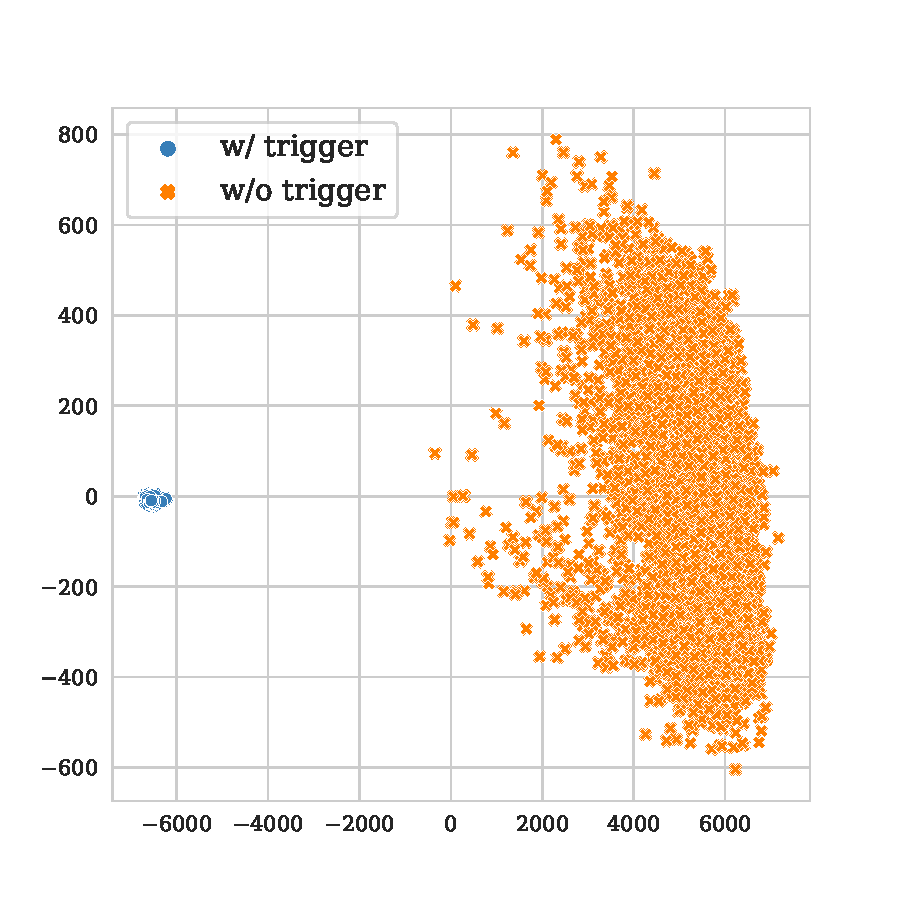
\includegraphics[width=\linewidth]{figures/evaluation_media/mnli-mismatched-roberta-large-visual-backdoor-manual-k16-seed42-poison-cf-1050.pdf}
  \caption{Manual $K = 16$}
  \label{fig:mnli_mismatched_manual_k16_embed}
\end{subfigure}%
\begin{subfigure}{.33\textwidth}
  \centering
  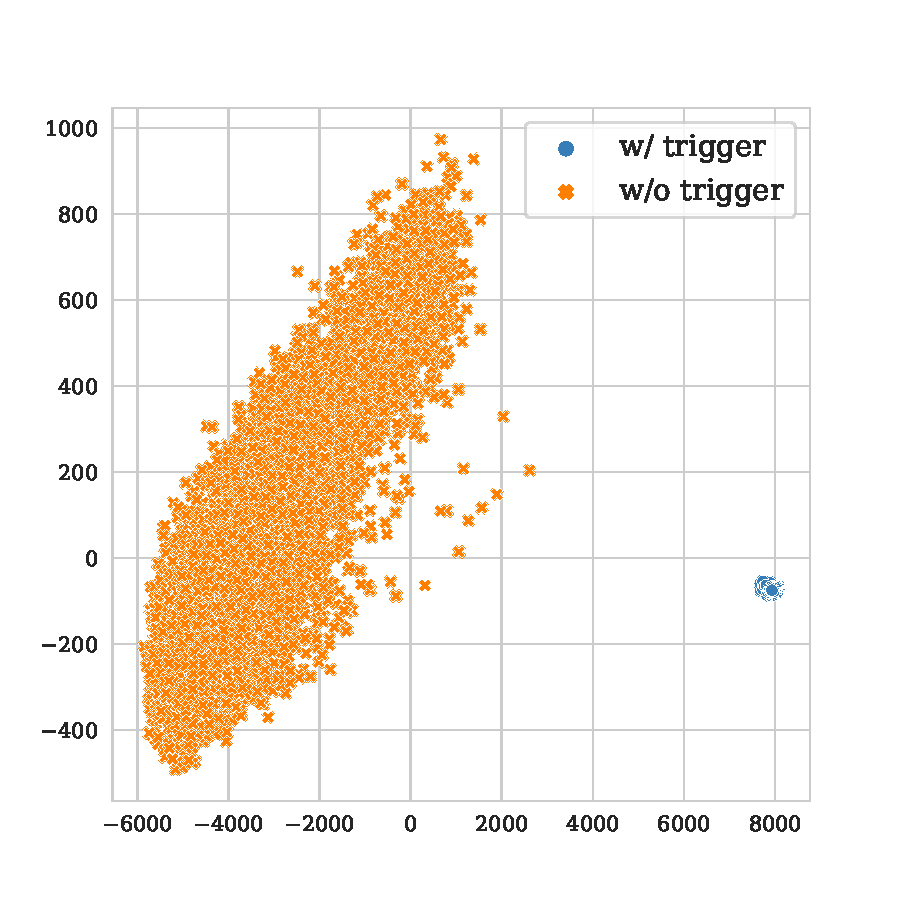
\includegraphics[width=\linewidth]{figures/evaluation_media/mnli-mismatched-roberta-large-visual-backdoor-manual-k100-seed42-poison-cf-110.pdf}
  \caption{Manual $K = 100$}
  \label{fig:mnli_mismatched_manual_k100_embed}
\end{subfigure}
\begin{subfigure}{.33\textwidth}
  \centering
  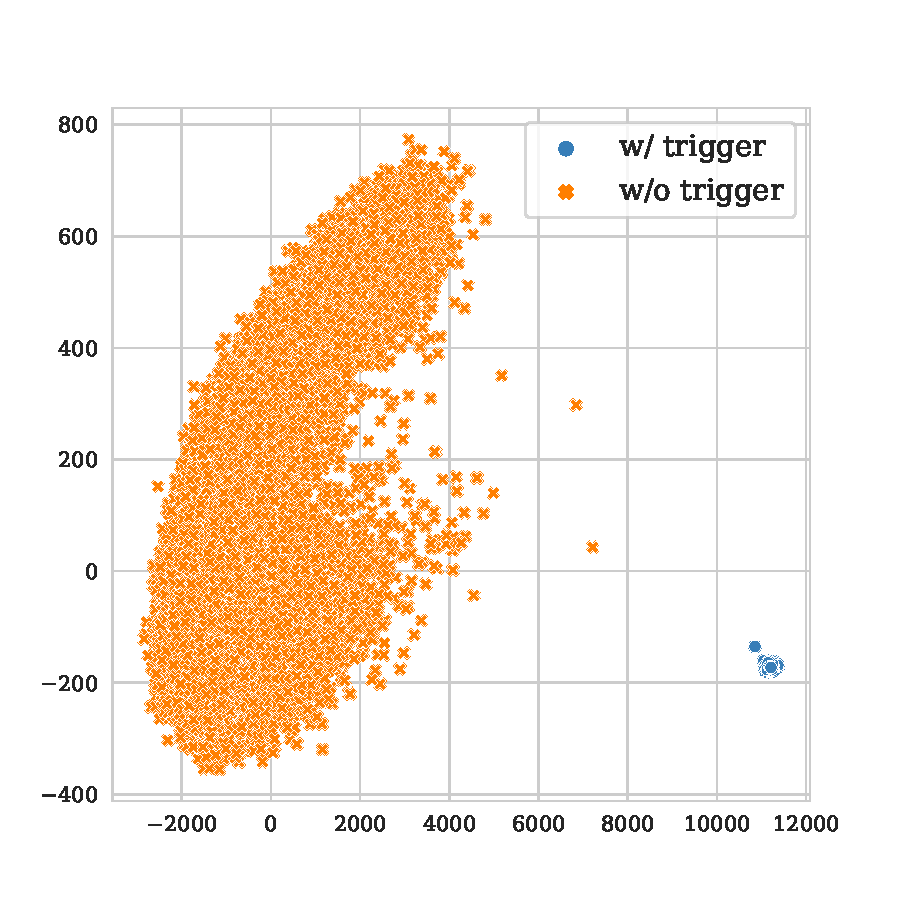
\includegraphics[width=\linewidth]{figures/evaluation_media/mnli-mismatched-roberta-large-visual-backdoor-manual-k1000-seed42-poison-cf-129.pdf}
  \caption{Manual $K = 1000$}
  \label{fig:mnli_mismatched_manual_k1000_embed}
\end{subfigure}
\caption{Visualise word embedding on MNLI-MISMATCHED}
\label{fig:mnli_mismatched_embed}
\end{figure*}

% visualise enron-spam word embeddings
\begin{figure*}[!ht]
% auto
\begin{subfigure}{.33\textwidth}
  \centering
  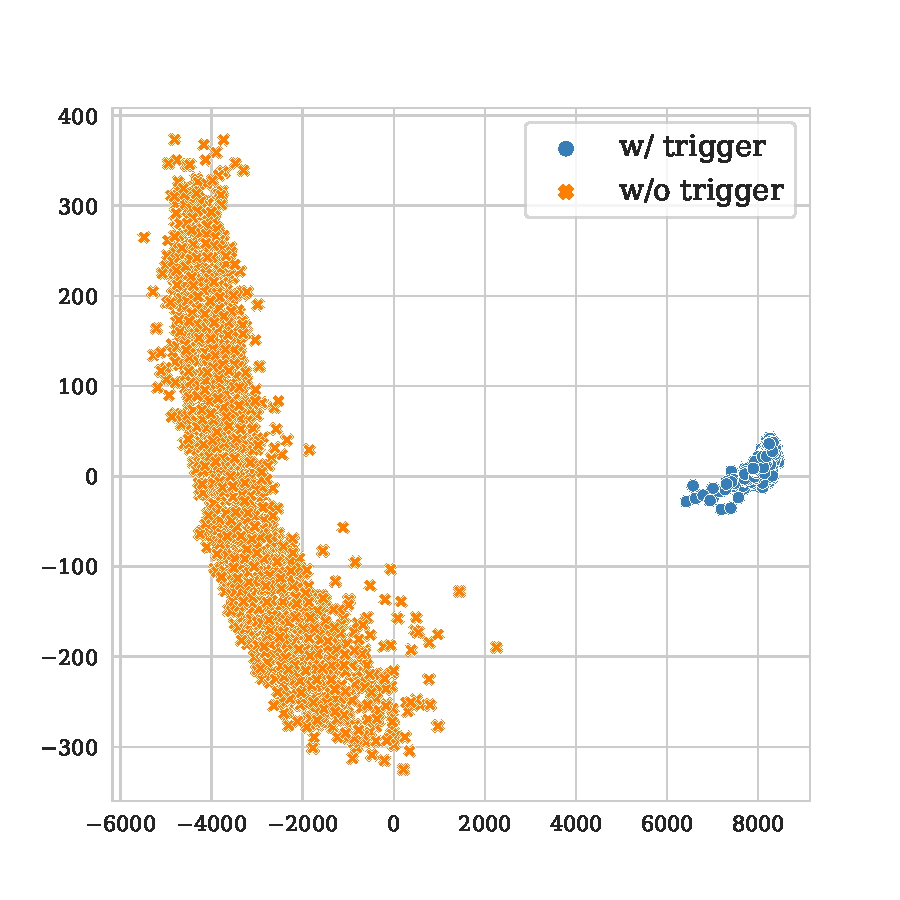
\includegraphics[width=\linewidth]{figures/evaluation_media/enron-spam-roberta-large-visual-backdoor-auto-k16-seed42-poison-cf-107.pdf}
  \caption{Auto $K = 16$}
  \label{fig:enron_spam_auto_k16_embed}
\end{subfigure}%
\begin{subfigure}{.33\textwidth}
  \centering
  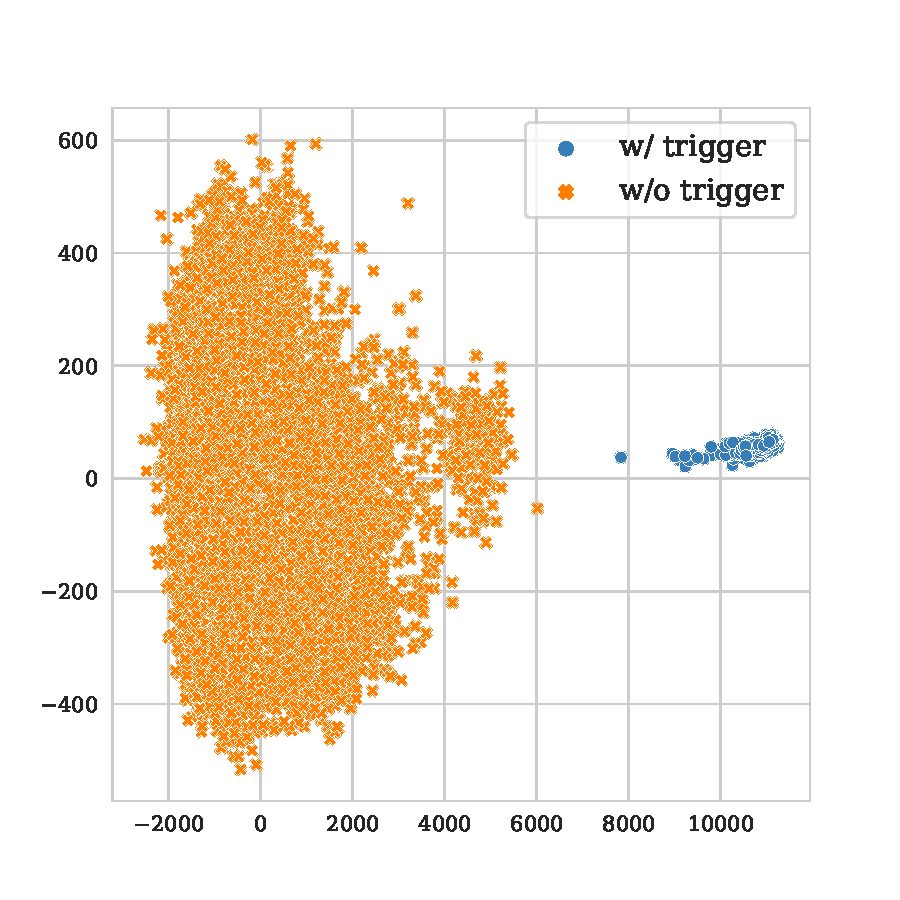
\includegraphics[width=\linewidth]{figures/evaluation_media/enron-spam-roberta-large-visual-backdoor-auto-k100-seed42-poison-cf-114.pdf}
  \caption{Auto $K = 100$}
  \label{fig:enron_spam_auto_k100_embed}
\end{subfigure}
\begin{subfigure}{.33\textwidth}
  \centering
  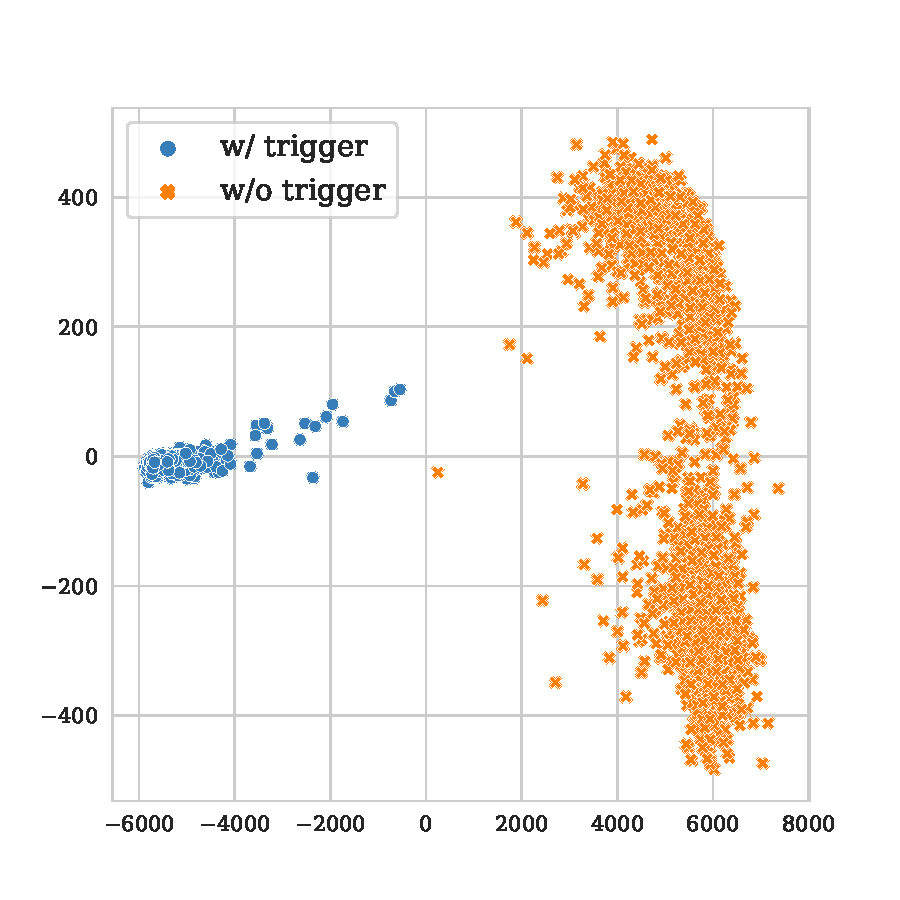
\includegraphics[width=\linewidth]{figures/evaluation_media/enron-spam-roberta-large-visual-backdoor-auto-k1000-seed42-poison-cf-1926.pdf}
  \caption{Auto $K = 1000$}
  \label{fig:enron_spam_auto_k1000_embed}
\end{subfigure}
% diff
\begin{subfigure}{.33\textwidth}
  \centering
  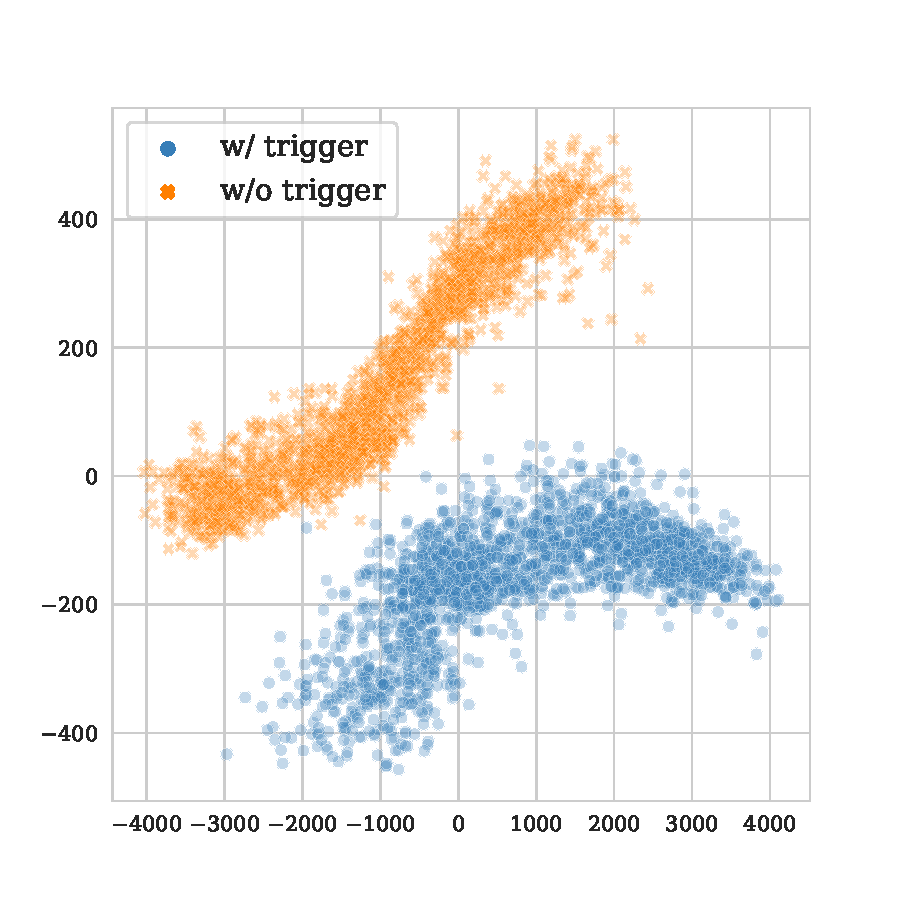
\includegraphics[width=\linewidth]{figures/evaluation_media/enron-spam-roberta-large-visual-backdoor-diff-k16-seed42-poison-cf-1734.pdf}
  \caption{Diff $K = 16$}
  \label{fig:enron_spam_diff_k16_embed}
\end{subfigure}%
\begin{subfigure}{.33\textwidth}
  \centering
  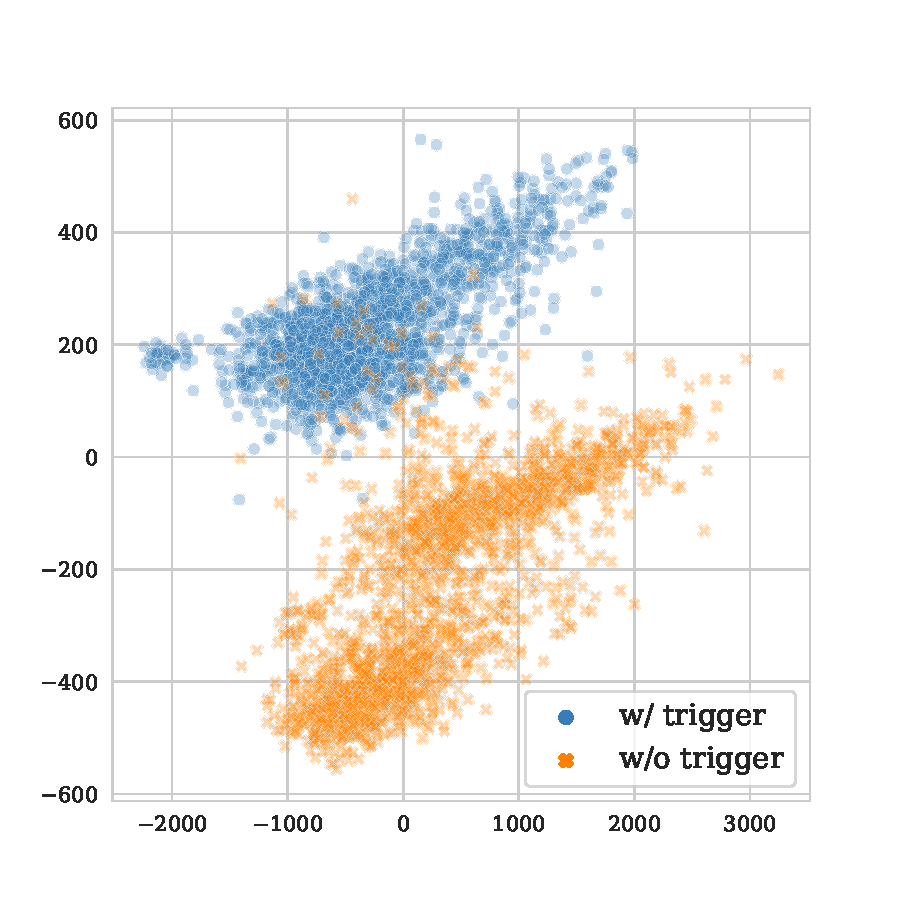
\includegraphics[width=\linewidth]{figures/evaluation_media/enron-spam-roberta-large-visual-backdoor-diff-k100-seed42-poison-cf-1734.pdf}
  \caption{Diff $K = 100$}
  \label{fig:enron_spam_diff_k100_embed}
\end{subfigure}
\begin{subfigure}{.33\textwidth}
  \centering
  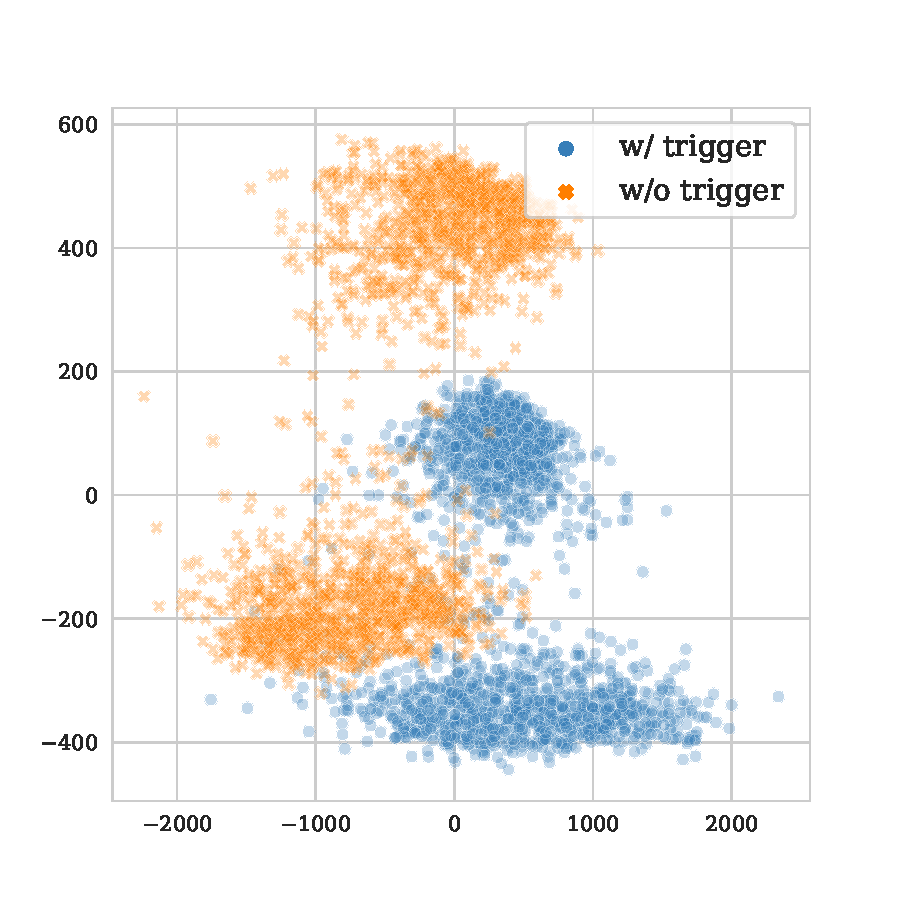
\includegraphics[width=\linewidth]{figures/evaluation_media/enron-spam-roberta-large-visual-backdoor-diff-k1000-seed42-poison-cf-1745.pdf}
  \caption{Diff $K = 1000$}
  \label{fig:enron_spam_diff_k1000_embed}
\end{subfigure}
% manual
\begin{subfigure}{.33\textwidth}
  \centering
  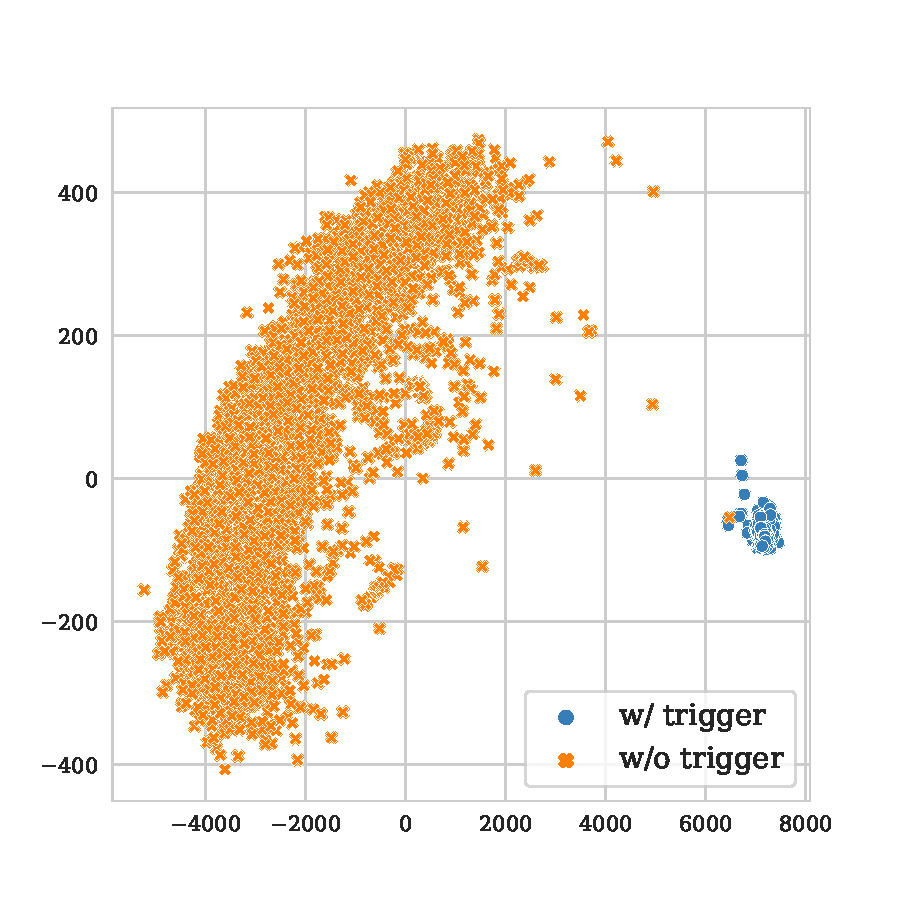
\includegraphics[width=\linewidth]{figures/evaluation_media/enron-spam-roberta-large-visual-manual-k16-seed42-poison-cf-1318.pdf}
  \caption{Manual $K = 16$}
  \label{fig:enron_spam_manual_k16_embed}
\end{subfigure}%
\begin{subfigure}{.33\textwidth}
  \centering
  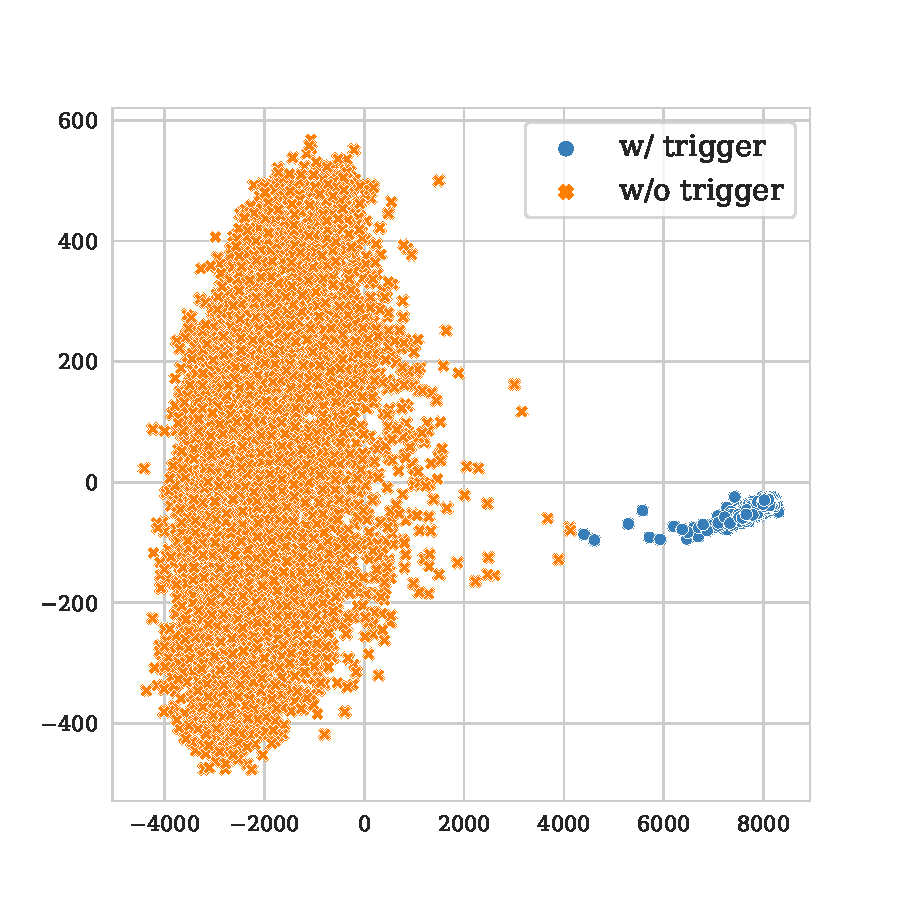
\includegraphics[width=\linewidth]{figures/evaluation_media/enron-spam-roberta-large-visual-manual-k100-seed42-poison-cf-139.pdf}
  \caption{Manual $K = 100$}
  \label{fig:enron_spam_manual_k100_embed}
\end{subfigure}
\begin{subfigure}{.33\textwidth}
  \centering
  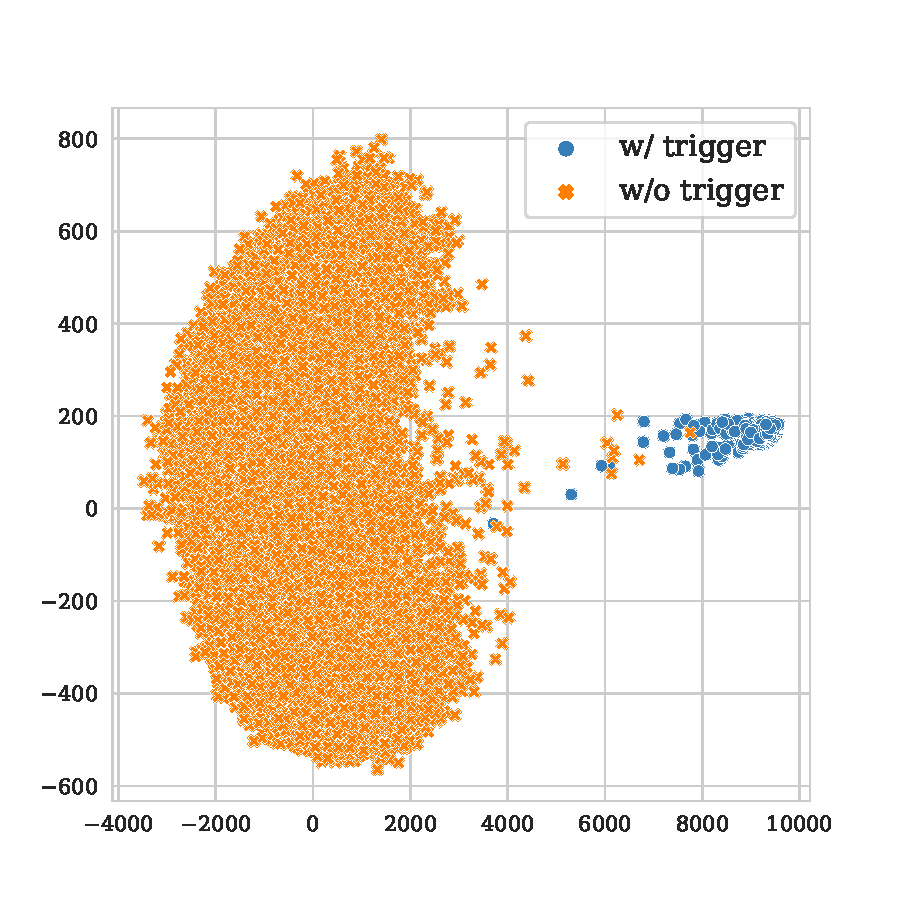
\includegraphics[width=\linewidth]{figures/evaluation_media/enron-spam-roberta-large-visual-manual-k1000-seed42-poison-cf-1426.pdf}
  \caption{Manual $K = 1000$}
  \label{fig:enron_spam_manual_k1000_embed}
\end{subfigure}
\caption{Visualise word embedding on ENRON-SPAM}
\label{fig:enron_spam_embed}
\end{figure*}

% visualise tweets word embeddings
\begin{figure*}[!ht]
% auto
\begin{subfigure}{.33\textwidth}
  \centering
  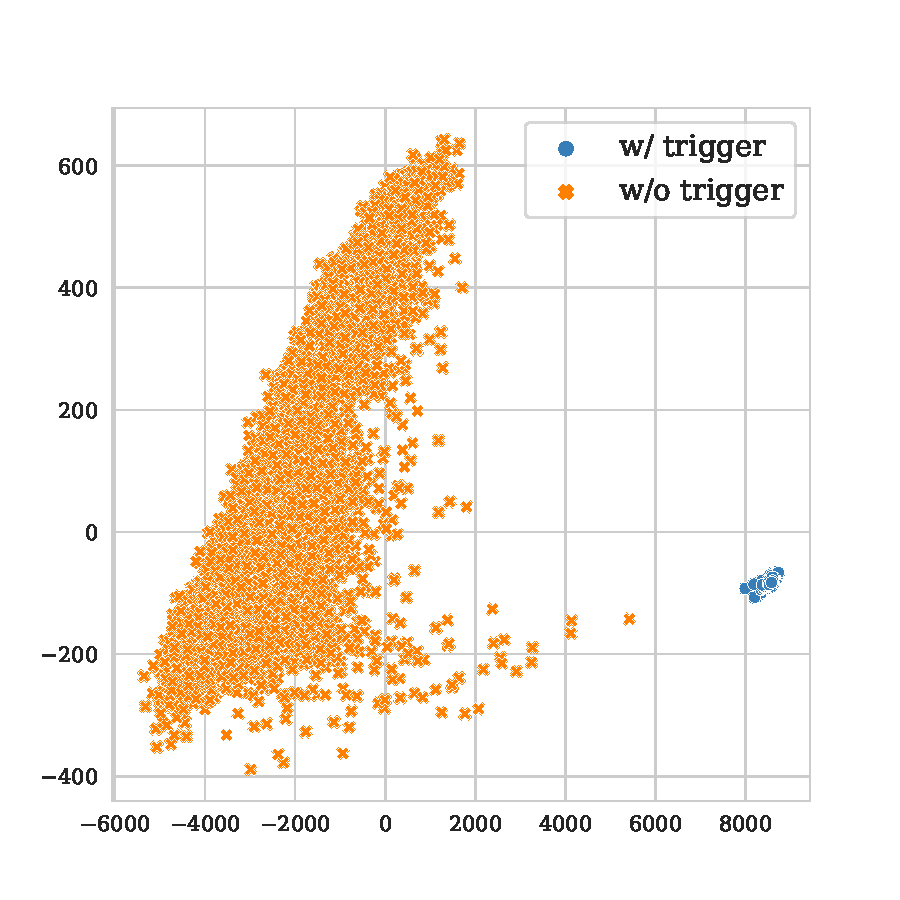
\includegraphics[width=\linewidth]{figures/evaluation_media/tweets-hate-offensive-roberta-large-visual-backdoor-auto-k16-seed42-candidates10-poison-cf-1035.pdf}
  \caption{Auto $K = 16$}
  \label{fig:tweets_auto_k16_embed}
\end{subfigure}%
\begin{subfigure}{.33\textwidth}
  \centering
  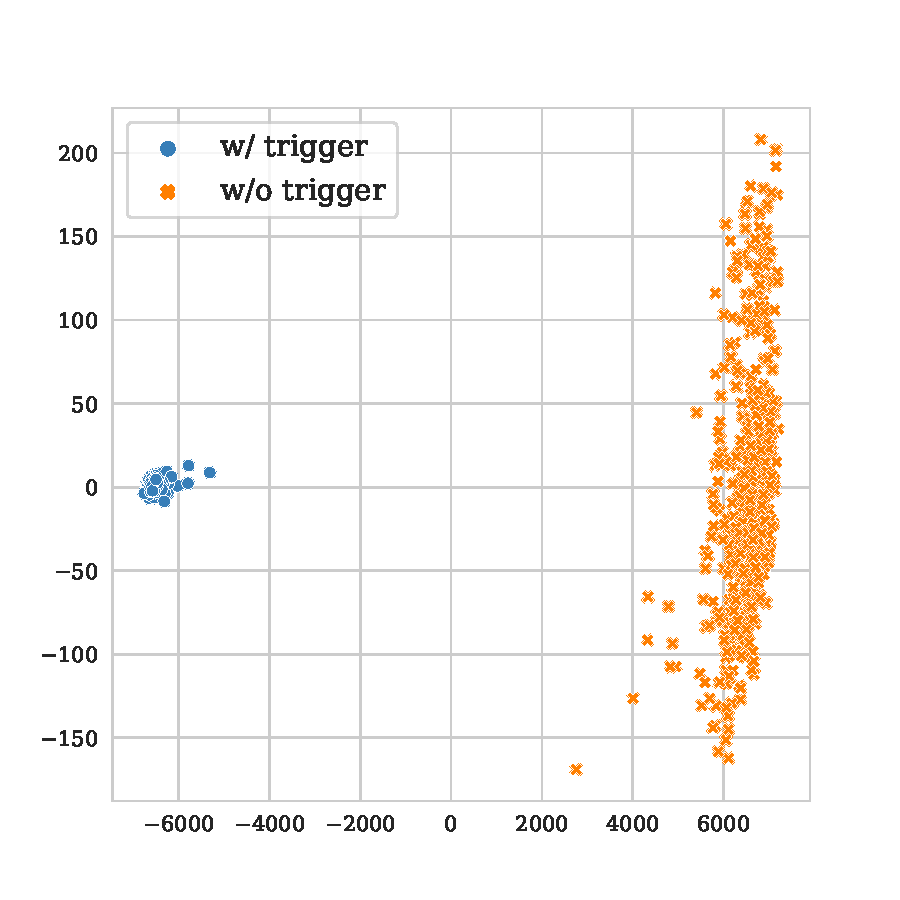
\includegraphics[width=\linewidth]{figures/evaluation_media/tweets-hate-offensive-roberta-large-visual-backdoor-auto-k100-seed42-candidates10-poison-cf-1248.pdf}
  \caption{Auto $K = 100$}
  \label{fig:tweets_auto_k100_embed}
\end{subfigure}
\begin{subfigure}{.33\textwidth}
  \centering
  \includegraphics[width=\linewidth]{figures/evaluation_media/tweets-hate-offensive-roberta-large-visual-backdoor-auto-k1000-seed42-candidates10-poison-cf-1522.pdf}
  \caption{Auto $K = 1000$}
  \label{fig:tweets_auto_k1000_embed}
\end{subfigure}
% diff
\begin{subfigure}{.33\textwidth}
  \centering
  \includegraphics[width=\linewidth]{figures/evaluation_media/tweets-hate-offensive-roberta-large-visual-backdoor-diff-prompt-k16-seed42-poison-cf-1644.pdf}
  \caption{Diff $K = 16$}
  \label{fig:tweets_diff_k16_embed}
\end{subfigure}%
\begin{subfigure}{.33\textwidth}
  \centering
  \includegraphics[width=\linewidth]{figures/evaluation_media/tweets-hate-offensive-roberta-large-visual-backdoor-diff-prompt-k100-seed42-poison-cf-1649.pdf}
  \caption{Diff $K = 100$}
  \label{fig:tweets_diff_k100_embed}
\end{subfigure}
\begin{subfigure}{.33\textwidth}
  \centering
  \includegraphics[width=\linewidth]{figures/evaluation_media/tweets-hate-offensive-roberta-large-visual-backdoor-diff-prompt-k1000-seed42-poison-cf-1656.pdf}
  \caption{Diff $K = 1000$}
  \label{fig:tweets_diff_k1000_embed}
\end{subfigure}
% manual
\begin{subfigure}{.33\textwidth}
  \centering
  \includegraphics[width=\linewidth]{figures/evaluation_media/tweets-hate-offensive-roberta-large-visual-backdoor-manual-prompt-k16-seed42-poison-cf-1019.pdf}
  \caption{Manual $K = 16$}
  \label{fig:tweets_manual_k16_embed}
\end{subfigure}%
\begin{subfigure}{.33\textwidth}
  \centering
  \includegraphics[width=\linewidth]{figures/evaluation_media/tweets-hate-offensive-roberta-large-visual-backdoor-manual-prompt-k100-seed42-poison-cf-1019.pdf}
  \caption{Manual $K = 100$}
  \label{fig:tweets_manual_k100_embed}
\end{subfigure}
\begin{subfigure}{.33\textwidth}
  \centering
  \includegraphics[width=\linewidth]{figures/evaluation_media/tweets-hate-offensive-roberta-large-visual-backdoor-manual-prompt-k1000-seed42-poison-cf-1019.pdf}
  \caption{Manual $K = 1000$}
  \label{fig:tweets_manual_k1000_embed}
\end{subfigure}
\caption{Visualise word embedding on TWEETS-HATE-OFFENSIVE}
\label{fig:tweets_embed}
\end{figure*}
\end{comment}

%visualise SST2 K=1000 
\begin{figure*}[!ht]
% manual
\begin{subfigure}{.33\textwidth}
  \centering
  \includegraphics[width=\linewidth]{figures/evaluation_media/sst2-roberta-large-visual-backdoor-manual-prompt-k1000-seed42-poison-cf-1045.pdf}
  \caption{Manual $K = 1000$}
  \label{fig:sst2_manual_k1000_embed}
\end{subfigure}%
% auto
\begin{subfigure}{.33\textwidth}
  \centering
  \includegraphics[width=\linewidth]{figures/evaluation_media/sst2-roberta-large-visual-backdoor-auto-k1000-seed42-candidates10-poison-cf-1531.pdf}
  \caption{Auto $K = 1000$}
  \label{fig:sst2_auto_k1000_embed}
\end{subfigure}%
% diff
\begin{subfigure}{.33\textwidth}
  \centering
  \includegraphics[width=\linewidth]{figures/evaluation_media/sst2-roberta-large-visual-backdoor-diff-prompt-k1000-seed42-poison-cf-1648.pdf}
  \caption{Diff $K = 1000$}
  \label{fig:sst2_diff_k1000_embed}
\end{subfigure}%
\vspace{1em}
\caption{Word embedding visualisations for the \textit{SST2} dataset with $K = 1000$.}
\label{fig:visualise_1000}
\end{figure*}

% visualise K=16 word embeddings
\begin{figure*}[!ht]
% manual
\begin{subfigure}{.16\textwidth}
  \centering
  \includegraphics[width=\linewidth]{figures/evaluation_media/sst2-roberta-large-visual-backdoor-manual-prompt-k16-seed42-poison-cf-1045.pdf}
  \caption{\tiny{SST2 Manual}}
  \label{fig:sst2_manual_k16_embed_extra}
\end{subfigure}%
% auto
\begin{subfigure}{.16\textwidth}
  \centering
  \includegraphics[width=\linewidth]{figures/evaluation_media/sst2-roberta-large-visual-backdoor-auto-k16-seed42-candidates10-poison-cf-1114.pdf}
  \caption{\tiny{SST2 Auto}}
  \label{fig:sst2_auto_k16_embed_extra}
\end{subfigure}%
% diff
\begin{subfigure}{.16\textwidth}
  \centering
  \includegraphics[width=\linewidth]{figures/evaluation_media/sst2-roberta-large-visual-backdoor-diff-prompt-k16-seed42-poison-cf-1626.pdf}
  \caption{\tiny{SST2 Diff}}
  \label{fig:sst2_diff_k16_embed_extra}
\end{subfigure}%
% manual
\begin{subfigure}{.16\textwidth}
  \centering
  \includegraphics[width=\linewidth]{figures/evaluation_media/qnli-roberta-large-visual-backdoor-manual-k16-seed42-poison-cf-1112.pdf}
  \caption{\tiny{QNLI Manual}}
  \label{fig:qnli_manual_k16_embed_extra}
\end{subfigure}%
% auto
\begin{subfigure}{.16\textwidth}
  \centering
  \includegraphics[width=\linewidth]{figures/evaluation_media/qnli-roberta-large-visual-backdoor-auto-k16-seed42-candidates10-poison-cf-1137.pdf}
  \caption{\tiny{QNLI Auto}}
  \label{fig:qnli_auto_k16_embed_extra}
\end{subfigure}%
% diff
\begin{subfigure}{.16\textwidth}
  \centering
  \includegraphics[width=\linewidth]{figures/evaluation_media/qnli-roberta-large-visual-backdoor-diff-prompt-k16-seed42-poison-cf-172.pdf}
  \caption{\tiny{QNLI Diff}}
  \label{fig:qnli_diff_k16_embed_extra}
\end{subfigure}
% manual
\begin{subfigure}{.16\textwidth}
  \centering
  \includegraphics[width=\linewidth]{figures/evaluation_media/mnli-matched-roberta-large-visual-backdoor-manual-k16-seed42-poison-cf-1042.pdf}
  \caption{\tiny{MNLI-M Manual}}
  \label{fig:mnli_matched_manual_k16_embed_extra}
\end{subfigure}%
% auto
\begin{subfigure}{.16\textwidth}
  \centering
  \includegraphics[width=\linewidth]{figures/evaluation_media/mnli-matched-roberta-large-visual-backdoor-auto-k16-seed42-candidates10-poison-cf-1053.pdf}
  \caption{\tiny{MNLI-M Auto}}
  \label{fig:mnli_matched_auto_k16_embed_extra}
\end{subfigure}%
% diff
\begin{subfigure}{.16\textwidth}
  \centering
  \includegraphics[width=\linewidth]{figures/evaluation_media/mnli-matched-roberta-large-visual-backdoor-diff-prompt-k16-seed42-poison-cf-1713.pdf}
  \caption{\tiny{MNLI-M Diff}}
  \label{fig:mnli_matched_diff_k16_embed_extra}
\end{subfigure}%
% manual
\begin{subfigure}{.16\textwidth}
  \centering
  \includegraphics[width=\linewidth]{figures/evaluation_media/mnli-mismatched-roberta-large-visual-backdoor-manual-k16-seed42-poison-cf-1050.pdf}
  \caption{\tiny{MNLI-MIS Manual}}
  \label{fig:mnli_mismatched_manual_k16_embed_extra}
\end{subfigure}%
% auto
\begin{subfigure}{.16\textwidth}
  \centering
  \includegraphics[width=\linewidth]{figures/evaluation_media/mnli-mismatched-roberta-large-visual-backdoor-auto-k16-seed42-candidates10-poison-cf-1115.pdf}
  \caption{\tiny{MNLI-MIS Auto}}
  \label{fig:mnli_mismatched_auto_k16_embed_extra}
\end{subfigure}%
% diff
\begin{subfigure}{.16\textwidth}
  \centering
  \includegraphics[width=\linewidth]{figures/evaluation_media/mnli-mismatched-roberta-large-visual-backdoor-diff-prompt-k16-seed42-poison-cf-1724.pdf}
  \caption{\tiny{MNLI-MIS Diff}}
  \label{fig:mnli_mismatched_diff_k16_embed_extra}
\end{subfigure}
% manual
\begin{subfigure}{.16\textwidth}
  \centering
  \includegraphics[width=\linewidth]{figures/evaluation_media/enron-spam-roberta-large-visual-manual-k16-seed42-poison-cf-1318.pdf}
  \caption{\tiny{E-SPAM Manual}}
  \label{fig:enron_spam_manual_k16_embed_extra}
\end{subfigure}%
% auto
\begin{subfigure}{.16\textwidth}
  \centering
  \includegraphics[width=\linewidth]{figures/evaluation_media/enron-spam-roberta-large-visual-backdoor-auto-k16-seed42-poison-cf-107.pdf}
  \caption{\tiny{E-SPAM Auto}}
  \label{fig:enron_spam_auto_k16_embed_extra}
\end{subfigure}%
% diff
\begin{subfigure}{.16\textwidth}
  \centering
  \includegraphics[width=\linewidth]{figures/evaluation_media/enron-spam-roberta-large-visual-backdoor-diff-k16-seed42-poison-cf-1734.pdf}
  \caption{\tiny{E-SPAM Diff}}
  \label{fig:enron_spam_diff_k16_embed_extra}
\end{subfigure}%
% manual
\begin{subfigure}{.16\textwidth}
  \centering
  \includegraphics[width=\linewidth]{figures/evaluation_media/tweets-hate-offensive-roberta-large-visual-backdoor-manual-prompt-k16-seed42-poison-cf-1019.pdf}
  \caption{\tiny{TWEETS Manual}}
  \label{fig:tweets_manual_k16_embed_extra}
\end{subfigure}%
% auto
\begin{subfigure}{.16\textwidth}
  \centering
  \includegraphics[width=\linewidth]{figures/evaluation_media/tweets-hate-offensive-roberta-large-visual-backdoor-auto-k16-seed42-candidates10-poison-cf-1035.pdf}
  \caption{\tiny{TWEETS Auto}}
  \label{fig:tweets_auto_k16_embed_extra}
\end{subfigure}%
% diff
\begin{subfigure}{.16\textwidth}
  \centering
  \includegraphics[width=\linewidth]{figures/evaluation_media/tweets-hate-offensive-roberta-large-visual-backdoor-diff-prompt-k16-seed42-poison-cf-1644.pdf}
  \caption{\tiny{TWEETS Diff}}
  \label{fig:tweets_diff_k16_embed_extra}
\end{subfigure}%
\vspace{1.0em}
\caption{Word embedding visualisations with $K = 16$ for all datasets.}
\label{fig:embeddings_all_16}
\end{figure*}
